\documentclass[prb,twocolumn]{revtex4-1}
\usepackage{times}
\usepackage{bbm}
\usepackage[dvips]{graphicx}
\usepackage{latexsym,amsmath,amssymb,bm,euscript}
\usepackage[dvips]{color}
\usepackage{multirow}
\usepackage{calligra}

\DeclareMathAlphabet{\mathcalligra}{T1}{calligra}{m}{n}
\DeclareFontShape{T1}{calligra}{m}{n}{<->s*[2.2]callig15}{}

%\newcommand{\scripty}[1]{\ensuremath{\mathcalligra{#1}}}
\newcommand{\scripty}[1]{w}

\def\ra{\rangle} % bra
\def\la{\langle} % ket
\def\uz{U(1)\times\mathbb{Z}_2}
\def\ztwo{\mathbb{Z}_2}
\def\ztwot{\mathbb{Z}_2^T}
\newcommand{\cp}{$CP^1$ }
\newcommand{\nccp}{$NCCP^1$}

\begin{document}

\title{Numerical Study of a Bosonic Topological Insulator}
\date{\today}
\pacs{}

\author{Scott D. Geraedts}
\author{Olexei I. Motrunich}
\affiliation{Department of Physics, California Institute of Technology, Pasadena, California 91125, USA}

%%%%%%%%%%%%%%%%%%%%%%%%%%%%%%%%%%%%%%%%%%%%%%%%%%%%%%%%%%%%%%%
\begin{abstract}
We study a topological phase of interacting bosons in $(3+1)$ dimensions which is protected by time-reversal and charge conservation symmetry. We present a precise model of bosons on a lattice which realizes this phase. The idea behind our model, which can be studied in sign-free Monte Carlo simulations, is to bind bosons to topological defects called hedgehogs. We determine the phase diagram of the model, and observe a Witten effect in the bulk which confirms that it is a bosonic topological insulator. We also study the boundary between the topological insulator and a trivial insulator. We find a surface phase diagram which includes exotic superfluids, a topologically ordered phase, and a phase with a Hall effect quantized to one-half of the value possible in a purely two-dimensional system. By binding multiple hedgehogs to each boson we also realize symmetry-enriched topologically-ordered phases.
\end{abstract}
%%%%%%%%%%%%%%%%%%%%%%%%%%%%%%%%%%%%%%%%%%%%%%%%%%%%%%%%%%%%%%%
\maketitle

\section{Introduction}
The study of topological phases of matter has been a major component of condensed matter research in recent decades. Among the many phases studied, the topological insulator (TI) is one of the most prominent. The TI is a three-dimensional phase of free fermions. Though it is insulating in the bulk, its topological behavior can be deduced from its unusual surface properties, in particular the odd number of Dirac cones it has on its surface. The topological insulator is an example of a symmetry-protected topological phase (SPT), like all SPT's, it has short-ranged entanglement, which implies that is has a unique ground state on any closed manifold. This is in contrast to intrinsically topologically ordered states like the fractional quantum Hall effect. The relevant symmetries for the topological insulator are charge conservation and time-reversal, and if either of these symmetries are broken it loses its topological properties.

One obvious extension of research into topological insulators is to consider the effects of interactions on their properties. This is however a difficult task. Many of the methods used to study TI's involve the properties of their band structure, and these methods obviously do not apply to the strongly interacting case. As an introduction to this difficult problem, one can try to study an analog of the topological insulator, constructed of interacting bosons instead of fermions. Certain theoretical techniques, like the Monte Carlo studies employed in this paper, work only for bosonic systems. In addition, in bosonic systems we know that the non-interacting case would be a condensate, so we can be sure that the topological behavior is due to the interactions.

The study of topological phases of interacting bosons is relatively recent, but much progress has been made. Chen, Liu, Gu, and Wen\cite{WenScience,*WenPRB} have used group cohomology theory to determine which symmetries and dimensions can lead to non-trivial topological phases. However, this approach tells us little about the properties of these phases, which must be determined through other methods. One well-studied case is that of SPT's in two dimensions with $U(1)$ symmetry. 
Lu and Vishwanath\cite{LuVishwanath} proposed a Chern-Simons field theory to describe both the bulk and edges of these systems and showed that such systems have a Hall effect quantized to an even integer, (in units of $e^2/h$) and possess gapless edge modes. Therefore such systems are called `bosonic quantum Hall phases'. 
Senthil and Levin\cite{SenthilLevin} showed how to access such phases in a quantum Hall-like setting by starting with two species of bosons and using flux attachment. 
In an earlier work, we provided an alternative exactly solvable model that replaces flux attachment with a binding of bosons to vortices, giving the bosons non-trivial statistics.
We studied this model in Monte Carlo and found a topological phase.\cite{FQHE}
%One drawback of the flux attachment technique is that it is not related to a microscopic model. To change this, in an earlier work we considered extending the symmetry to $U(1)\times U(1)$, i.e.~ two different species of bosons. Flux from one species of boson was bound to charge from the other species, and vice versa. In this way, we obtained a microscopic model which realized the bosonic quantum Hall effect, and studied this model in Monte Carlo.\cite{FQHE} 

Interacting bosonic topological phases which are analogs of the topological insulator in three dimensions can also be considered. Senthil and Vishwanath\cite{SenthilVishwanath} have found effective field theories which can describe both the bulk and the surface of a three-dimensional `bosonic topological insulator' with charge conservation and time-reversal symmetry. They find exotic behavior on the surface of their system which can be used to assert the topological behavior in the bulk. 

In particular, Senthil and Vishwanath find three kinds of exotic phases on the surface of the bosonic TI. These surface phases cannot exist in a purely two-dimensional system and their existence on the surface of a three-dimensional system shows that the system is topological. The first kind of phase is a superfluid, which breaks charge conservation symmetry. There are actually several different types of superfluids which can exist on the surface. The gapped excitations in these superfluids have fractional charge and statistics which cannot exist in a purely two-dimensional system.  Phase transitions between the different superfluids are predicted to be deconfined critical points. Another surface phase breaks time-reversal symmetry on the surface. This phase has a Hall conductivity quantized to one-half of the value possible in a purely two-dimensional system. Since the Hall conductivity in a bosonic quantum Hall effect is quantized to even integers, this surface phase is expected to have an odd integer Hall conductivity. Finally, it is possible to have a surface phase which breaks no symmetries but has intrinsic topological order of a kind impossible in a purely two-dimensional system with these symmetries.

In both the two- and three-dimensional cases, the topological behavior can be thought of as coming from the binding of bosons to point topological defects. In two dimensions the topological defects were vortices, and the binding is essentially an exact realization of the flux attachment. In three dimensions the topological defects are hedgehogs.
Bulk field theories for the bosonic TI can be constructed by adding an additional $SO(3)$ symmetry to the model, and binding hedgehogs of this symmetry to the bosons.\cite{SenthilVishwanath} Metliski and Fisher produced a construction which explicitly binds hedgehogs to bosons and showed that it leads to the same topological phase. In that case the hedgehogs can be shown to come from the bosons themselves.\cite{Max} 

In this work, we construct explicit models which realize the interacting bosonic analog of the topological insulator. The models have both charge conservation symmetry, and a $\ztwot$ symmetry to be discussed in the main text. They can be studied in Monte Carlo simulations. The main idea behind our constructions is the binding of hedgehogs to bosons, and condensation of the resulting bound states. We introduce addition `spin' degrees of freedom into our model, it is from these spins that hedgehogs will be defined. We present two different models which realize this physics. In the first model, described in Section \ref{section::Heisenberg}, the spins are represented by $SO(3)$ degrees of freedom with Heisenberg interactions. We introduce a term in our action which energetically binds hedgehogs to bosons, and we show that this term can lead to a phase (which we call the `binding phase') which is a condensate of these bound states.

In order to show that the binding phase is indeed the bosonic topological insulator, we will attempt to find the phases predicted by Senthil and Vishwanath on its surface. Initially we find only superfluids on the surface. In our Monte Carlo simulations, we do not have access to the statistics of the gapped excitations of the model. Therefore we cannot determine whether the superfluids we observe are the exotic superfluids predicted by Senthil and Vishwanath, or more conventional superfluids. We find that the surface superfluids in our model are connected by a direct transition. If this transition were second-order, then it would be a deconfined phase transition as predicted. However, we cannot access large enough system sizes to determine the order of the observed phase transition. 

We can try to find other exotic surface phases by explicitly breaking the $\ztwot$ symmetry of our model on the surface. If the bulk of the system is in a topological phase, this will lead to a Hall conductivity quantized to an odd integer. In order to measure this Hall conductivity in our system, we need to introduce external electromagnetic fields. In the model in Section \ref{section::Heisenberg}, this is complicated by our definition of hedgehog number, which is a discontinuous function of the Heisenberg spins. When the external fields are introduced, the action becomes a discontinuous function of these fields, which prevents us from measuring the surface Hall conductivity.

To remedy this, in Section \ref{section::CP1} we introduce a second model which binds hedgehogs to bosons. In this model, we represent the spins with an easy-plane \cp model.
Hedgehogs can be identified with the monopoles of the gauge field of this \cp model. This formulation will allow us to make several measurements which demonstrate that our phase is a bosonic topological insulator.

One measurement that we can make is called the Witten effect.\cite{MaxWitten,Max} This is the binding of one-half of a boson charge to external monopoles We introduce external monopoles into the bulk of our system and find that they bind to precisely half of a charge.

We then determine the surface phases of our model. We again find superfluids connected by a direct transition.  We can also break the $\ztwot$ symmetry on the surface. In the \cp model, we can measure the Hall conductivity and we find it to be quantized to odd integers as predicted. We reiterate that this Hall conductivity cannot be observed in a purely two-dimensional model, and so we must be measuring the Hall conductivity on the surface of a topological phase. Finally, we also find a phase which breaks none of the symmetries of the model. We suspect that this phase has intrinsic topological order, but we do not know how to test this using Monte Carlo.

In Monte Carlo studies of the `bosonic quantum Hall' phases, we found that we can obtain symmetry-enriched phases with intrinsic topological order by binding multiple topological defects to bosons. In Section \ref{section::multiple} we consider such a binding in $(3+1)$ dimensions. We find that binding of multiple topological defects leads to a bulk phase with intrinsic topological order.

%%%%%%%%%%%%%%%%%%%%%%%%%%%%%%%%%%%%%%%%%%%%%%%%%%%%%%%%%%%%%%%%%%%%%%%%%%%%%%%%%%%%%%%%%%%%%%%5
\section{Realizing the topological insulator by binding bosons to hedgehogs of $SO(3)$ spins}
\label{section::Heisenberg}

We first study the binding between topological defects and bosons by using hedgehogs of a Heisenberg model as our topological defects. We demonstrate the existence of a phase which is a condensate of bound states of hedgehogs and bosons, and explore its properties. This model provides an intuitive introduction to the physics of binding topological defects to bosons. 

\subsection{Bulk Phase Diagram}
\label{subsec::bulkheis}
We study the following action, in (3+1)-D Euclidean space-time:
\begin{equation}
S=S_{\rm spin}+\frac{\lambda}{2}\sum_{r,\mu} [ J_\mu(r)- Q_\mu(r)]^2.
\label{action}
\end{equation}
$S_{\rm spin}$ is an action which controls fluctuations in the $SO(3)$ spins. The second term describes the binding between bosons and hedgehogs. The bosons are represented by integer-valued conserved currents, $J_\mu(r)$, defined on the links of a four-dimensional cubic lattice, where $r$ is the position on the lattice and $\mu\in (x,y,z,\tau)$ is a direction. These currents represent the world-lines of the bosons in the (3+1) dimensional space-time. The $Q_\mu$ variables represent the hedgehogs, which are also integer-valued conserved currents.  When the real number $\lambda$ is large, this term will bind bosons and hedgehogs together. We work with periodic boundary conditions, and require no net charge and no net hedgehog number, so that the $J_\mu$ and $Q_\mu$ currents have winding number zero.

In this section we represent the spin degrees of freedom by $SO(3)$ unit vectors. For $S_{\rm spin}$, we take the following action, which describes a Heisenberg model:
\begin{equation}
S_{\rm spin}=-\beta\sum_{R,\mu} \vec{n}(R)\cdot \vec{n}(R+\mu).
\end{equation}
Here $\vec{n}=(n_a,n_b,n_c)$ are three-component unit vectors which represent the spins. They reside on a different lattice from the $J_\mu$ and $Q_\mu$ variables above. This lattice has its sites labelled by $R$, and they are located at the centers of the (hyper)cubes of the lattice in Eq.~(\ref{action}). 
%more details about this?

From these ${\vec{n}(R)}$, we can define the hedgehog current $Q_\mu$ using the prescription in Refs.~\onlinecite{LesikAshvin} and \onlinecite{SachdevHedgehogs}, modified to four dimensions. We summarize this prescription here. One first defines variables $\alpha_\mu(R)$, which exist on links connecting the spins $\vec{n}_i\equiv\vec n(R)$ and $\vec{n}_j\equiv\vec n(R+\mu)$:
\begin{equation}
e^{i\alpha_{\mu}(R)}=\frac{1+\vec{n}_i\cdot\vec{n}_j+\vec{n}_i\cdot\vec{N}_0+\vec{n}_j\cdot\vec{N}_0+i\vec{N}_0 \cdot(\vec{n}_i\times\vec{n}_j)}{\sqrt{2(1+\vec{n}_i\cdot\vec{n}_j)(1+\vec{n}_i\cdot\vec{N}_0)(1+\vec{n}_j\cdot\vec{N}_0})}.
\label{alpha}
\end{equation}
Here $\vec{N}_0$ is a reference vector which we can choose arbitrarily. 
We then define placket ``fluxes'' $\omega_{\mu\nu}\in (-\pi,\pi]$ as follows:
\begin{equation}
\omega_{\mu\nu}(R)={\rm floor}[\nabla_\nu\alpha_\mu(R)-\nabla_\mu\alpha_\nu(R)].
\label{omega}
\end{equation}
Here $\nabla_\nu \alpha_\mu(R)\equiv \alpha_\mu(R+\nu)-\alpha_\mu(R)$. One can show that changing the reference vectors $\vec{N}_0$ corresponds to a gauge transformation of the $\alpha$ variables so that $\omega_{\mu\nu}$ is independent of the reference vector. Finally, we can define the hedgehog current:
\begin{equation}
Q_\mu(r)=\frac{1}{4\pi}\epsilon_{\mu\nu\rho\sigma}\nabla_{\nu} \omega_{\rho\sigma}(R).
\label{monopoledef}
\end{equation}
Consider for example 
\begin{equation}
Q_\tau[r=R+(\frac{1}{2},\frac{1}{2},\frac{1}{2},-\frac{1}{2})]=\frac{1}{2\pi}[\nabla_x\omega_{yz}+\nabla_y\omega_{zx}+\nabla_z\omega_{xy}].
\end{equation}
If we consider only three dimensions of our four-dimensional lattice, $Q_\tau$ is defined at a point in the center of a cube in the $x,y,z$ directions. The $\omega$ variables are the fluxes passing through the center of this cube, and so the hedgehog is equal to the net flux out of the cube.
% the $\omega_{\mu\nu}$ involved in the definition of $Q_\mu$ make up a cube on the lattice indexed by $R$. We have defined the lattices so that there is a vertex of the lattice labelled by $r$ at the center of this cube, and this is where the $Q_\mu$ variables are defined. 
When all four dimensions are considered, $Q_\tau$ becomes a link in the $\tau$ direction.  

The above action can be studied in Monte Carlo. In addition to simple independent updates of $\vec{n}$ and $J_\mu$, when $\lambda$ is large one needs to try updates which change both $J_\mu$ and $Q_\mu$ in such a way that the second term in Eq.~(\ref{action}) is unchanged. To do this we choose a spin and an amount to update it, and check to see if any $Q_\mu$ variables will change as a result of this update. If so we attempt to update $J_\mu$ and $\vec{n}$ simultaneously.

In this work, we monitor the ``internal energy per site'', $\epsilon= S /{\rm Vol}$, where ${\rm Vol}\equiv L^4$ is the volume of the system, which has linear size $L$. From this, we can determine the specific heat:
\begin{equation}
C=(\la \epsilon^2\ra-\la\epsilon\ra^2)\times{\rm Vol}.
\end{equation}
We can locate phase transitions in our model by looking for singularities in the specific heat. We also monitor the magnetization per spin:
\begin{equation}
m=\la |\sum_R \vec{n}(R)|\ra/{\rm Vol}.
\end{equation}
When the spins are disordered, the average of the magnetization is proportional to $1/\sqrt{\rm Vol}$. Therefore we can use measurements of magnetization at different sizes to determine if the spins are ordered.

To study the behavior of the boson currents, we monitor current-current correlators, defined as:
\begin{equation}
\rho_J({k})=\la J_\mu({k})J_\mu(-{k})\ra
\label{rho}
\end{equation}
where $k$ is a wave vector and 
\begin{equation}
J_\mu({k})\equiv\frac{1}{\rm \sqrt{Vol}}\sum_r J_\mu(r)e^{-i{k}\cdot r}.
\end{equation}
In the space-time isotropic system, $\rho_J({k})$ is independent of the direction $\mu$, and when we show numerical data we average over all directions to improve statistics. We evaluate the correlators at the smallest non-zero ${k}$, i.e.~if $\mu$ is in the $x$ direction, we average over ${k}_{min}=(0,\frac{2\pi}{L},0,0)$, $(0,0,\frac{2\pi}{L},0)$, and $(0,0,0,\frac{2\pi}{L})$. We also monitor the current-current correlators of the hedgehog currents, $\rho_Q(k)$, which are defined in the same way as for the boson currents.

In the phase where the $J_\mu$ are gapped, only small loops contribute to the current-current correlators and $\rho_J(k_{\rm min})\sim {k}_{\rm min}^2=1/L^2$, while when the $J_\mu$ proliferate $\rho_J$ is independent of system size. Therefore we can use finite-size scaling of this quantity to determine the locations of phase transitions. For the hedgehog currents, $\rho_Q(k_{\rm min})\sim {k}_{\rm min}^2$ in all phases, so we cannot use finite-size scaling of these variables to find phase transitions. 

To understand the bulk phase diagram of this model analytically, it is convenient to define new variables
\begin{equation}
\tilde J_\mu(r)=J_\mu(r)-Q_\mu(r).
\label{shift}
\end{equation}
Expressed in these variables, the first and second terms in Eq.~(\ref{action}) decouple, and we can study them independently. 
At small $\beta$, the $\vec{n}$ spins are disordered, which also implies that the hedgehog currents are proliferated. As $\beta$ is increased, the spins order. This means that there is a large energy cost for hedgehog currents to exist. We say that the hedgehog currents are gapped, and only small loops of them are present. We can determine the location of the spin-ordering phase transition by finding singularities in the heat capacity, or by performing finite-size scaling on the magnetization as described above. The value found by our numerics agrees with the literature.\cite{McKenzie2}

At small $\lambda$, the $\tilde J_\mu$ variables are proliferated. In our original variables, this means that the boson currents are independent of the hedgehog currents. At large $\lambda$, the $\tilde J_\mu$ variables are gapped. The boson currents are bound to the hedgehog currents. The result of this can be seen in Fig.~\ref{heisbulk}, which shows the current-current correlators for the boson and hedgehog currents. For small $\lambda$, there is no relation between the bosons (red solid line) and the hedgehogs (blue dashed line). As $\lambda$ is increased, the current-current correlators become essentially identical as the bosons and hedgehogs are bound together. We can determine the location of the phase transition in $\lambda$ by studying singularities in the heat capacity, or by peforming finite-size scaling on $\rho_{\tilde J}$ as described above. The inset in Fig.~\ref{heisbulk} shows the phase diagram. At small $\lambda$ and $\beta$, both the boson and hedgehog currents proliferate and are not bound. At small $\lambda$ and large $\beta$ hedgehog currents are gapped, but boson currents proliferate, while at large $\lambda$ and $\beta$ all currents are gapped. When $\lambda$ is large and $\beta$ is small the system is in the `binding' phase, which we will argue is a $(3+1)$d topological phase protected by the appropriate symmetry.

\begin{figure}
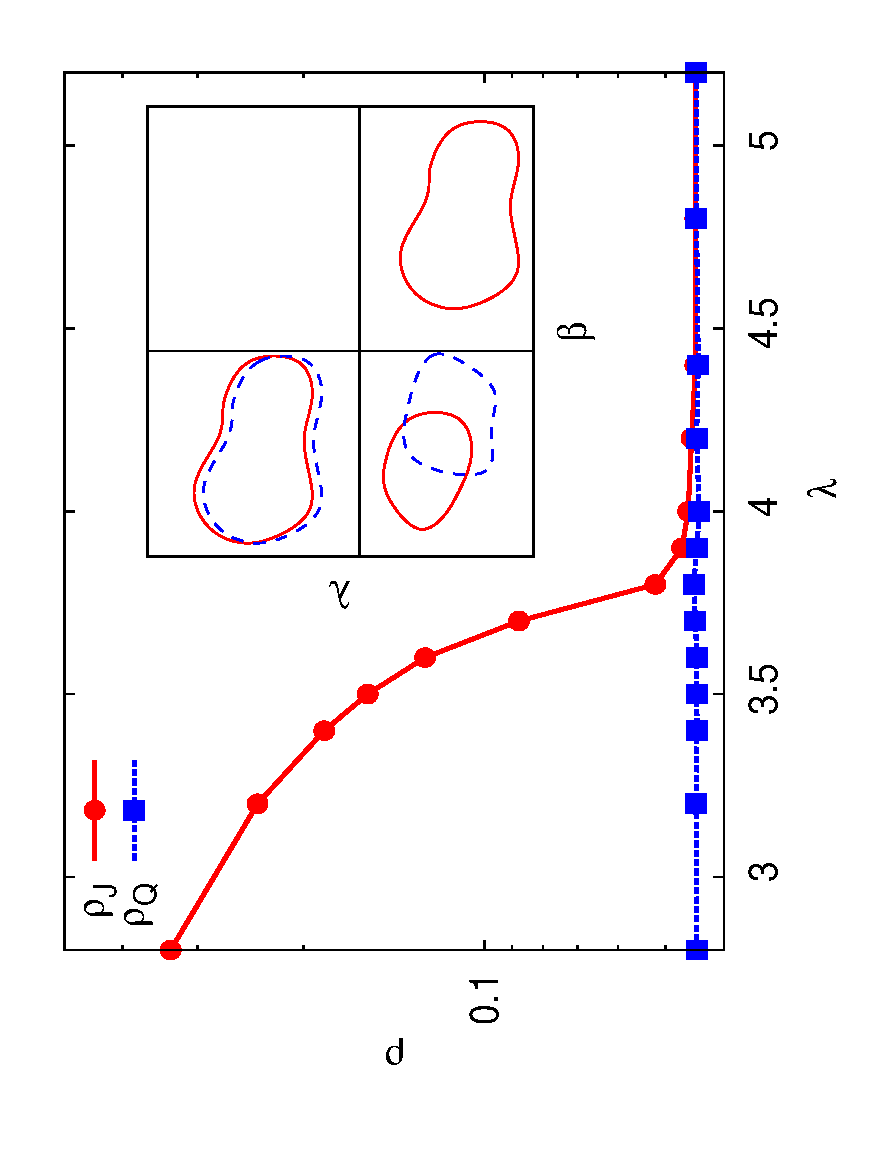
\includegraphics[angle=-90,width=\linewidth]{figures/heisbulkout.eps}
\caption{Inset: Bulk phase diagram for the model in Eq.~(\ref{action}) with Heisenberg spins and bosons. (the phase diagram is mathematically equivalent to a system of decoupled currents and spins, hence the straight line boundaries) At $\lambda=0$, the system has a paramagnet-ferromagnet transition as $\beta$ is increased, while the bosons are superfluid throughout. As $\lambda$ is increased, the boson currents bind to the hedgehog currents. The loops in the phases show a `snapshot' of the phase. Red solid loops mean that boson currents are proliferated in the phase, while blue dashed loops indicate proliferated hedgehog currents. The phase of interest is the `binding' phase in the upper left phase where bosons are bound to hedgehogs. The main figure shows the current-current correlations of the bosons and hedgehogs as $\lambda$ is increased while $\beta=0$. We see that the correlators become essentially equal as the system enters the upper left phase, indicating that bosons have bound to hedgehogs.}
\label{heisbulk}
\end{figure}

It is also helpful to think about the `easy-plane' regime for the spin variables, in which the spins, $\vec{n}$, are roughly in the $ab$-plane, with only small $c$ components. In the easy-plane case we can define `vortices' of the $U(1)$ spins which are the $ab$-components of the $\vec n$ variables. 
The vortices are defined on the plackets of the cubic lattice. Therefore in the $(3+1)$d space-time they are represented as two-dimensional `world-sheets'. When dealing with vortices, one can gain intuition by thinking in terms of only the three spatial dimensions of our (3+1) dimensional space-time. In this picture the bosons and hedgehogs are represented by point particles, while the vortices are represented by lines. The results of the next several paragraphs can be most easily understood by thinking in this picture.

Though ordinary $U(1)$ spins are not defined at the core of a vortex, our spins have a $c$-component which can point either up or down at the vortex core. We can define two species of vortices, which we call the $\uparrow$ and $\downarrow$ species, depending on whether $n_c$ is positive or negative. This description is useful since an $\uparrow$ vortex on top of a $\downarrow$ vortex is a hedgehog. Therefore our system can be thought of as a system of vortex lines of two different species. These vortex lines can change species, and the locations where this happens are hedgehogs. This is illustrated in Fig.~\ref{monopoles}.

Hedgehog number can be either positive or negative, and this is determined by the properties of the vortex line the hedgehog is attached to. 
We can determine these relations by considering the behavior of our model under reflections of the spins in the $ab$ and $ac$ planes. (these symmetries are discussed in more detail in the following section)
Reflection in the $ab$-plane interchanges $\uparrow$ and $\downarrow$ vortex lines. On the other hand reflection in the $ac$-plane changes the vorticity of the vortex lines, from clockwise to counter-clockwise and vice-versa. Both of these operations negate the hedgehog number.
Let us define a positive hedgehog to be one which turns an $\uparrow$ vortex into a $\downarrow$ vortex, on a clockwise vortex line (pictured third from left in Fig.~\ref{monopoles}). The charges of other hedgehogs can be determined from the above symmetries, and are shown in Fig.~\ref{monopoles}. 

\begin{figure}
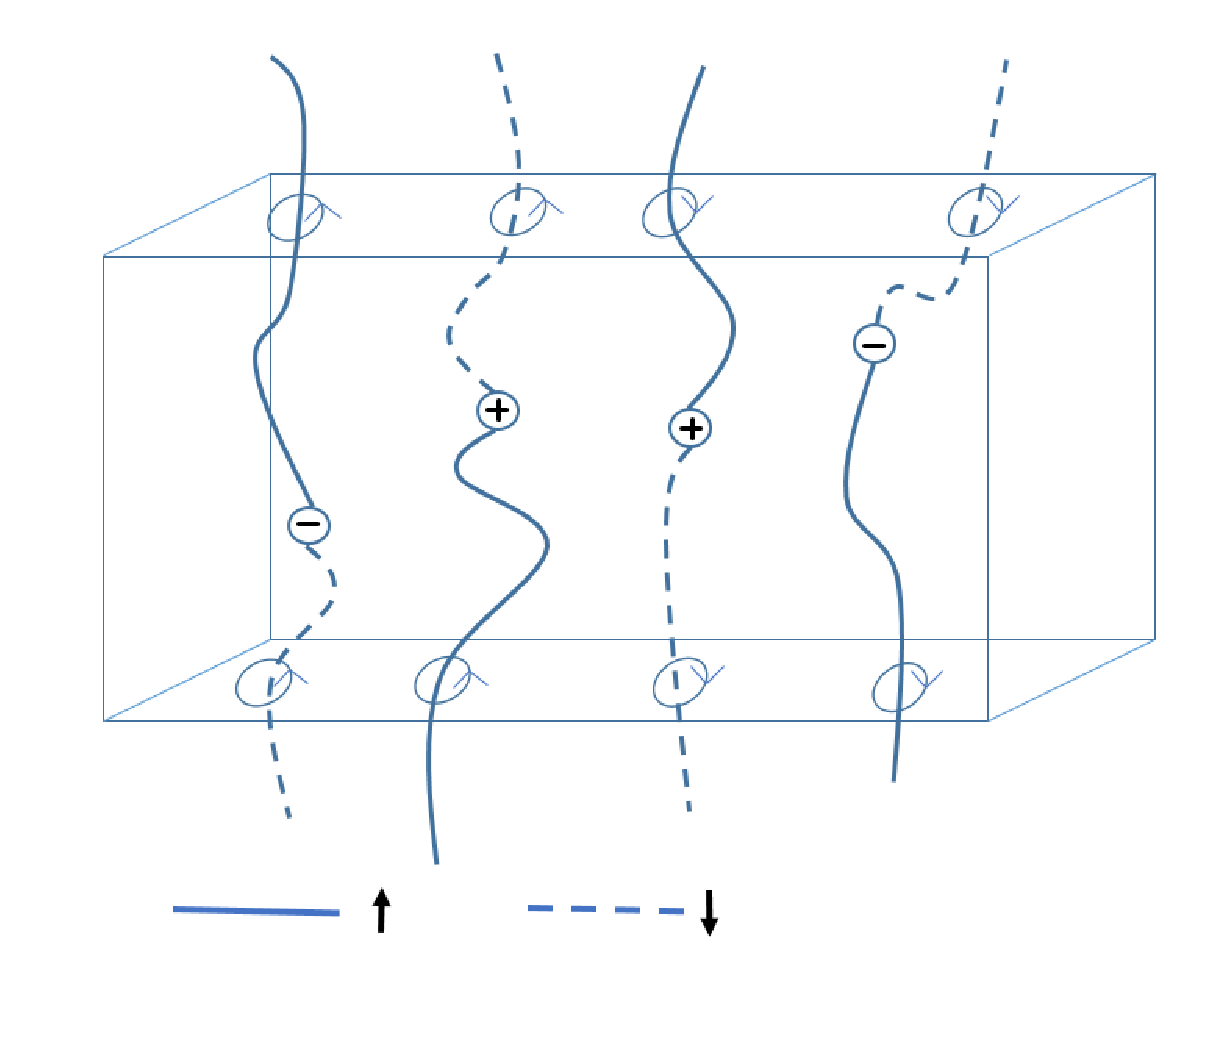
\includegraphics[width=\linewidth]{figures/monopoles.eps}
\caption{As discussed in the text, the easy-plane spin system has two species of vortex lines, $\uparrow$ and $\downarrow$. A hedgehog is a transition point between the two types of lines, with the sign of the hedgehog determined by the orientation of type and vorticity of the vortex lines, as shown with examples. This figure shows only the spatial dimensions of the system, therefore the hedgehogs are point particles and the vortices are lines. Applying a Zeeman field to the surface means allowing only one type of vortex line through the surface. This leads to a correlation between the hedgehog charge (and therefore the boson charge) and the vorticity at the surface, which is the origin of the Hall conductivity. }
\label{monopoles}
\end{figure}

%%%%%%%%%%%%%%%%%%%%%%%%%%%%%%%%%%%%%%%%%%%%%%%%%%%%%%%%%%%%%%%%%%%5
\subsubsection{Importance of Discrete Symmetry}

The action in Eq.~(\ref{action}) has a $U(1)$ symmetry which comes from the conservation of the $J_\mu$ currents; this is boson charge conservation symmetry. It also has an $SO(3)$ symmetry from the spins. Both of these symmetries protect the topological phase, in the sense that if they are broken it is possible to continuously connect the topological phase to a topologically trivial phase.
In addition, the action has 
a $\ztwo$ symmetry, which is obtained by reflecting the $\vec{n}$ spins around a plane. To see how this affects the hedgehog current, we can examine Eq.~(\ref{alpha}), taking the reference vector $N_0$ to be in the plane of reflection. We see that reflecting the spin changes the sign of the imaginary part of $e^{i\alpha_\mu}$, and therefore the hedgehog current changes sign under such a reflection. For our entire action to be invariant, we therefore need to combine such reflections with an operation which changes the sign of the boson currents. For concreteness and we will consider the $\ztwo$ symmetry corresponding to reflections in the $ab$ plane of the $\vec{n}$ variables. In this case the $\ztwo$ symmetry can be summarized as:
\begin{equation}
\begin{array}{ccc}
n_a,n_b & \rightarrow & n_a,n_b \\
n_c & \rightarrow & -n_c\\
Q_\mu & \rightarrow & -Q_\mu\\
J_\mu & \rightarrow & -J_\mu 
\end{array}.
\label{ztwoeqn}
\end{equation}
Note that it is also possible to reflect the $\vec n$ spins around a different plane, but this is not a distinct symmetry since it is simply the product of the above $\ztwo$ symmetry and an element of $SO(3)$. 

By analogy with the topological insulator, we would expect the $\ztwo$ symmetry described above to be a `time-reversal' symmetry, i.e.~it should be anti-unitary. Note that Eq.~(\ref{action}) is a real, $(d+1)$-dimensional action which is assumed to arise from the Trotter decomposition of a $d$-dimensional quantum Hamiltonian. The symmetry operations in Eq.~(\ref{ztwoeqn}) can be derived from the action of a symmetry operation on the quantum Hamiltonian. Therefore asking whether the symmetry in Eq.~(\ref{ztwoeqn}) is anti-unitary is the same as asking whether the symmetry of the quantum Hamiltonian which generates Eq.~(\ref{ztwoeqn}) is anti-unitary. This is a difficult question for us to answer as we do not know the quantum Hamiltonian which has Eq.~(\ref{action}) as its Trotter decomposition. We can imagine the case where the bosons are not bound to hedgehogs (this is a topologically trivial example). In this case we do know the quantum Hamiltonian, and we find that the symmetry operation which generates Eq.~\ref{ztwoeqn} is anti-unitary. Therefore it is likely that the $\ztwo$ symmetry we are considering is anti-unitary, and can be thought of as a time-reversal symmetry. From now on this symmetry will be denoted by $\ztwot$.

The action in Eq.~(\ref{action}) is invariant under several $\ztwo$ symmetries, but we expect that only the $\ztwot$ symmetry described above is important, as it protects the topological behavior. To see this we can break this symmetry and argue that the topological phase is destroyed.
We break the $\ztwot$ symmetry by introducing a Zeeman field into our action:
\begin{equation}
S_{\rm Zeeman}=-h\sum_R n_c(R).
\label{Zeeman}
\end{equation}
Here $h$ is the strength of the Zeeman field, which points in the $c$-direction. In our picture of two species of vortices (Fig.~\ref{monopoles}), the Zeeman field forbids one of the species. Since the vortex lines cannot change species, hedgehogs are forbidden and the binding phase is destroyed. 
This can be made more clear if we replace the binding term in Eq.~(\ref{action}) with the following term:
\begin{equation}
\frac{\lambda}{2}\sum_{r,\mu} [ J_\mu(r)- \eta Q_\mu(r)]^2.
\label{tbind}
\end{equation}
where $\eta$ is a real number. The introduction of $\eta$ allows us to tune the system between the trivial insulator ($\eta=0$)  and the binding phase ($\eta=1$). Without a Zeeman field, the system undergoes a phase transition as $\eta$ is changed between $0$ and $1$. 
When a Zeeman field is applied, hedgehogs are absent and so we can tune $\eta$ without going through a phase transition, and so the phase with $\eta=1$ is not distinct from the trivial insulator.
(Note that when $\eta=1$, the change of variables in Eq.~(\ref{shift}) uncouples the bosons and spins, so there is no phase transition upon making $h$ arbitrarily large. We can then tune $\eta$ to zero and finally reduce $h$ back to zero, all without undergoing a phase transition)

%%%%%%%%%%%%%%%%%%%%%%%%%%%%%%%%%%%%%%%%%%%%%%%%%%%%%%%%%%%%%%%%%%%5
\subsubsection{Binding of Multiple Bosons to a Hedgehog}
The above methods also allow us to answer the question of what happens to the system if $\eta$ is an integer larger than 1.  In a $U(1)\times U(1)$ system in two dimensions, we studied the binding of multiple bosons to vortices and found that each number of bound vortices led to a different symmetry-protected topological phase. There were therefore an integer number of SPTs.\cite{FQHE} In the present three-dimensional case the classification of Chen et al.\cite{WenScience,*WenPRB} predicts the existence of only one symmetry protected topological phase with this symmetry and in (3+1) dimensions. In agreement with this, we find that all systems with $\eta$ an even integer are topologically trivial, while when $\eta$ odd we have the same topological phase as $\eta=1$. 

We can justify this claim by showing that $\eta=2$ can be continuously connected to $\eta=0$ (which is a trivial insulator). This argument can then be extended to show that any two systems where $\eta$ differs by $2$ are in the same phase.
We start by considering two copies of our action, in the Heisenberg model and with $\eta=1$:
\begin{eqnarray}
&&S=-\beta\sum_{R,\mu}\left[ \vec{n}^{(1)}(R)\cdot \vec{n}^{(1)}(R+\mu)+\vec{n}^{(2)}(R)\cdot \vec{n}^{(2)}(R+\mu)\right]\nonumber\\
&&+\frac{\lambda}{2}\sum_{r,\mu}\left( [ J_\mu^{(1)}(r)- Q_\mu^{(1)}(r)]^2+[ J_\mu^{(2)}(r)- Q_\mu^{(2)}(r)]^2\right),
\label{doubleaction}
\end{eqnarray}
where the superscripts indicate which copy a variable is from, and we add the following terms:
\begin{eqnarray}
\delta S&=&-A\sum_{R} \vec{n}^{(1)}(R)\cdot \vec{n}^{(2)}(R)\nonumber\\
&-&B\sum_{r,\mu} \cos[\Phi^{(1)}(r)-\Phi^{(2)}(r)].
\label{AB}
\end{eqnarray} 
When $A$ is large and positive, the first term above locks spins of different types together, $\vec{n}^{(1)}\approx\vec{n}^{(2)}$. The hedgehog variables therefore take on the same values, and the either can be viewed as the spin system's hedgehog number in this case: $Q\approx Q^{(1)}\approx Q^{(2)}$. On the other hand, when $A$ is large and negative the spins of different types are locked in opposite directions, and $Q^{(1)}\approx-Q^{(2)}$. 
The $\Phi$ variables can be thought of as conjugates to the $J_\mu$ variables. More precisely, in our path integral we usually sum over only the configurations of $J_\mu$ in which the currents are divergenceless. We can instead sum over all configurations of $J_\mu$, and include the following term in our path integral:
\begin{equation}
\int_0^{2\pi} D\Phi e^{-i\sum_r (\sum_\mu\nabla_\mu J_\mu)\Phi(r)}
\end{equation}
which dynamically enforces the constraint that the boson currents be conserved. We introduce $\Phi$ variables for each copy of the boson currents, and the $B$ term is tunnelling between the two copies. 
When $B$ is large only the total of $J^{(1)}$ and $J^{(2)}$ is conserved and therefore we can identify the two copies of currents.

When $A$ and $B$ are large and positive, we can expand the terms on the second line of Eq.~(\ref{doubleaction}), and take $J=J^{(1)}+J^{(2)}$, $Q=Q^{(1)}=Q^{(2)}$. We are left with Eq.~(\ref{tbind}) with $\eta=2$. When $A$ is large and negative, but $B$ is still large and positive, $J$ is unchanged but the hedgehog number is zero as contributions from $Q^{(1)}$ and $Q^{(2)}$ cancel. This gives Eq.~(\ref{tbind}) with $\eta=0$.
% We see that when $A$ and $B$ are large, the hedgehog currents are \emph{added} ($Q^{\rm tot}_\mu=Q_\mu^1+Q_\mu^2$), while the boson currents are \emph{identified} ($J^{\rm tot}_\mu=J^1_\mu=J^2_\mu$). Therefore in this case Eq.~(\ref{doubleaction}) reduces to Eq.~(\ref{tbind}) with $\eta=2$. Furthermore, 
We can continuously deform $A=0$, $B=0$ to $A=\infty$, $B=\infty$ without undergoing a phase transition. In addition, we can deform $A=0$, $B=0$ to $A=-\infty$, $B=\infty$ without undergoing a phase transition. This implies that we can tune from $\eta=0$ to $\eta=2$ without undergoing a phase transition, and so both of these cases are in the trivial insulating phase.


%%%%%%%%%%%%%%%%%%%%%%%%%%%%%%%%%%%%%%%%%%%%%%%%%%%%%%%%%%%%%%%%%5
\subsection{Phase Diagram on the Boundary Between the Binding Phase and a Trivial Insulator}
\label{subsec:heissurf}
By analogy to the fermionic topological insulator, we expect that one way to investigate the topological nature of our phase is to study the physics of its surface. In particular, a number of interesting phases have been predicted on the surface of the bosonic TI,\cite{SenthilVishwanath} and if we can identify these phases on the surface of our binding phase it will be a powerful argument that the binding phase is a bosonic TI.

We introduce a surface between the binding phase and a trivial insulator by allowing $\eta$ in Eq.~(\ref{tbind}) to vary spatially.
%using a spatially varying function $\eta(r)$ so that Eq.~(\ref{action}) becomes:
%\begin{equation}
%S=S_{\rm spin}+\sum_r \frac{\lambda}{2}[J_\mu(r)-\eta(r) Q_\mu(r)]^2.
%\end{equation}
We vary $\eta$ in the $z$ direction, so that:
\begin{equation}
\eta(r)=
\left\{ \begin{array}{cc}
1 & z_L\leq z<z_R\\
0 & \rm{otherwise}\\
\end{array}\right..
\end{equation}
This leads to the binding phase in the region $z_L<z_R<z_R$, while the trivial phase occupies the rest of the space. Note that there are two surfaces of the binding phase: one at $z_L$ and one at $z_R$.

On the surface, we can measure all of the quantities which we measured in the bulk, but we now only sum over the sites near the surface, and when averaging over all directions we only use the $x$, $y$ and $\tau$ directions. 

The binding between hedgehogs and bosons in the bulk of the topological phase leads to exotic physics on the surface. In both the binding and trivial phase, hedgehog currents proliferate, while boson currents are bound to the hedgehog currents in the binding phase and are absent in the trivial phase, as shown in Fig.~\ref{surface}. Consider what happens when a hedgehog loop tries to cross the boundary between the phases. Since the boson currents must form closed loops, the above conditions cannot both be satisfied without something interesting happening on the surface. For example, we could have unbound boson currents on the surface, or hedgehogs could be forbidden from crossing the surface.



\begin{figure}
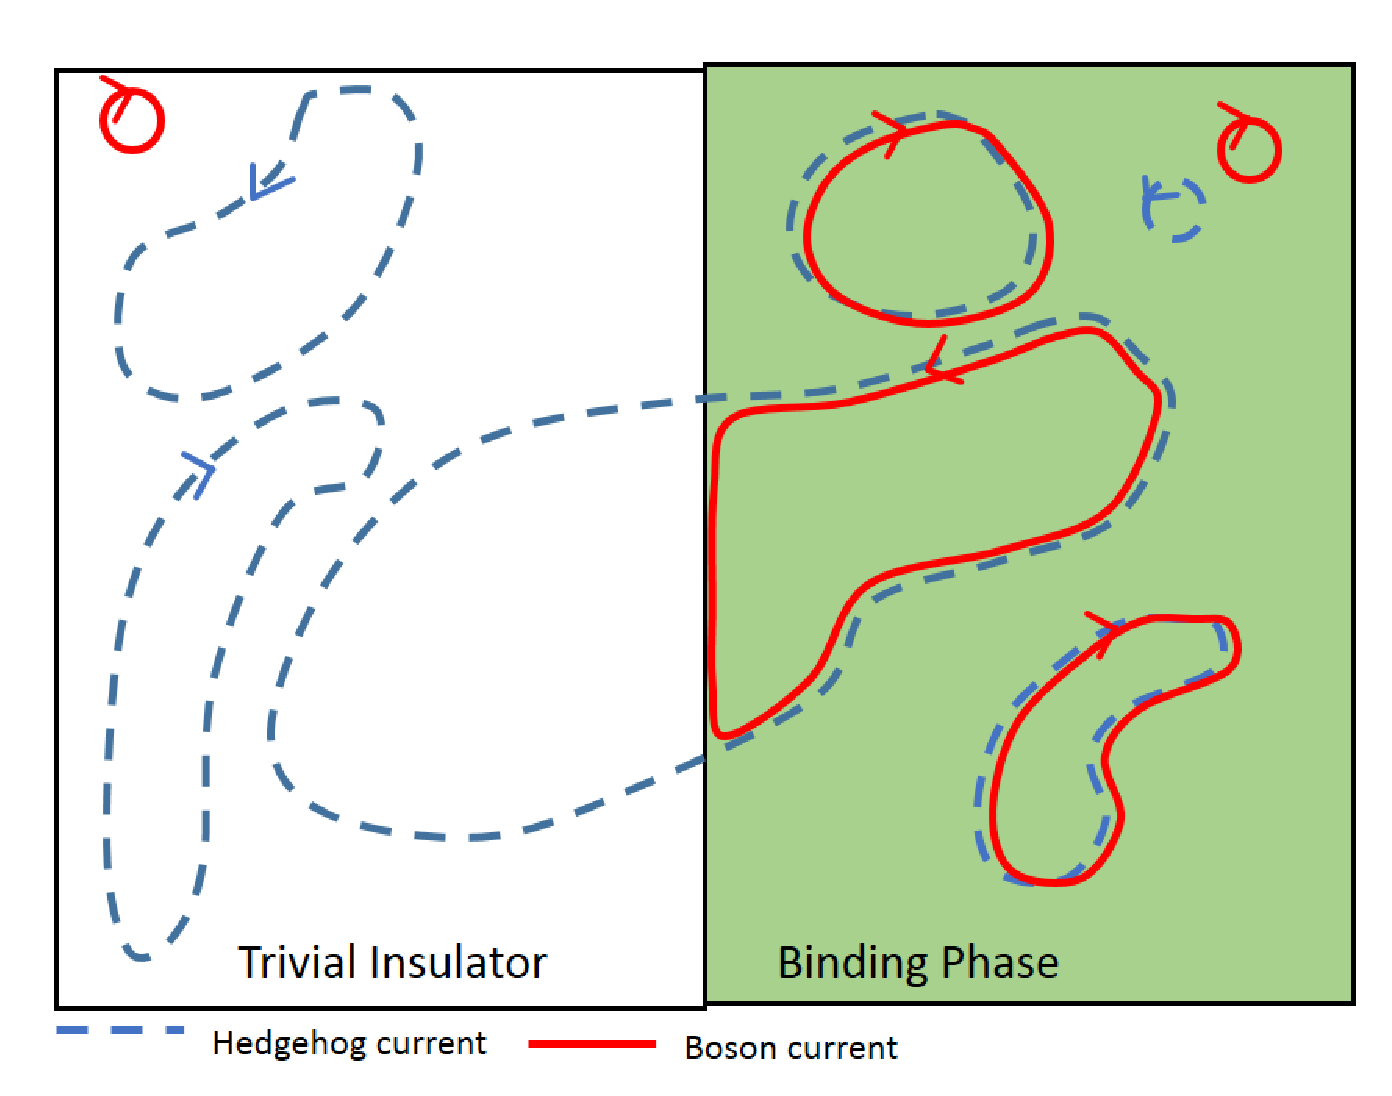
\includegraphics[width=\linewidth]{figures/surface.eps}
\caption{A snapshot of the system, when it is spatially divided into a region which is a trivial insulator and a region which is in the binding phase. In the trivial phase, boson currents are gapped and hedgehog currents are proliferated. In the binding phase both currents are gapped individually, but they form bound states which proliferate. Large hedgehog current loops can exist in either region, but when such a loop tries to cross the boundary the conservation of boson current leads to a conflict between the two sides and this can lead to exotic surface physics. }
\label{surface}
\end{figure}

In order to search for the predicted exotic surface behavior, we first determine the surface phase diagram.
To do this, we fix the values of $\beta$ and $\lambda$ in the bulk and tune them only on the surface, by setting:
\begin{equation}
\begin{array}{c}
\beta_\mu(X,Y,z-\frac{1}{2},T)\\
\lambda_\mu(x,y,\tau,z)\end{array}=
\left\{
\begin{array}{cc}
\beta_{\rm surf},\lambda_{\rm surf} & z=z_R,~\mu=\hat{x},\hat{y},\hat{\tau}\\
\beta_{\rm bulk},\lambda_{\rm bulk} & {\rm otherwise }
\end{array}\right.
\label{bulkvsurf}
\end{equation}
We obtain the phase diagram in the inset of Fig.~\ref{heissurf}, which contains three distinct phases. When $\lambda_{\rm surf}$ is small the bosons are in a superfluid phase, breaking their $U(1)$ symmetry. This is the scenario pictured in Fig.~\ref{surface}, where hedgehogs can cross the surface, and these crossings are connected by boson currents. If $\beta_{\rm surf}$ is also small the $SO(3)$ symmetry is unbroken as the spins are disordered. As $\beta_{\rm surf}$ increases the $SO(3)$ symmetry breaks, and so both symmetries are broken. At large $\lambda_{\rm surf}$ bosons see a large energy cost, and so the $U(1)$ symmetry is unbroken. This forbids hedgehogs from crossing the surface, leading to a system of $SO(3)$ spins with hedgehogs forbidden, which is known to break the $SO(3)$ symmetry.\cite{LauDasgupta} All data was taken with $\beta_{\rm bulk}=0$, $\lambda_{\rm bulk}=5.2$, parameters which put the bulk deep into the binding phase.

\begin{figure}
\includegraphics[angle=-90,width=0.9\linewidth]{figures/heissurf.eps}
\caption{The inset shows the phase diagram of the surface of the Heisenberg version of the model, without a Zeeman field. It was obtained by tuning the bulk into the phase where bosons and hedgehogs are bound, and then tuning $\beta$ and $\lambda$ {\em only on the surface}.  We find that our surface always spontaneously breaks  a symmetry. At small $\beta_{\rm surf}$ and $\lambda_{\rm surf}$ the $U(1)$ symmetry breaks and the bosons condense into a superfluid, while at large $\lambda_{\rm surf}$ the $SO(3)$ symmetry breaks and the spins align into a ferromagnet. At small $\lambda_{\rm surf}$ and large $\beta_{\rm surf}$ both symmetries are broken.  The main plot shows surface magnetization on a sweep in $\lambda_{\rm surf}$ for $\beta_{\rm surf}=0$. We show $mL^{3/2}$, which is independent of system size in the disordered phase, and grows with system size in the ordered phase. We can clearly see that the $SO(3)$ symmetry breaks as $\lambda_{\rm surf}$ is increased. All data in this section was taken with $\beta_{\rm bulk}=0$, $\lambda_{\rm bulk}=5.2$.}
\label{heissurf}
\end{figure}

The locations of the phases and phase transitions in Fig.~\ref{heissurf} were determined by studying singularities in the specific heat, as well as by studying the surface magnetization and current-current correlators. As an example of such data, in the main plot of Fig.~\ref{heissurf} we show the magnetization, multiplied by the square-root of the volume of the surface ($L^{3/2}$). This quantity should be constant when the spins are disorderd and should grow with system size when they are ordered. The data was taken with $\beta_{\rm surf}=0$ and increasing $\lambda_{\rm surf}$. We can see that the spins order at $\lambda_{\rm surf}\approx4$. 

In order to use the current-current correlators on the surface to detect the breaking of the $U(1)$ boson symmetry, we must treat the finite-size scaling carefully. 
The argument that $\rho_J\sim 1/L^2$ relied on the conservation of $J_\mu$, and this is no longer true if we consider only the surface, as currents can enter and exit from the rest of the system. Therefore we instead measure the current-current correlators in the entire system. (though only in the $x$, $y$, and $\tau$ directions) When currents are gapped everywhere, this quantity will still be proportional to $1/L^2$. If the surface is a superfluid, the current-current correlators will be independent of system size on the surface, but the volume of the surface is $1/L$ times the volume of the bulk. In Fig.~\ref{slabcurs} we plot $\rho_J\cdot L^2$. We see that at large $\lambda_{\rm surf}$ this quantity is independent of system size, which tells us that the currents are gapped everywhere and the surface is a trivial insulator in the boson degrees of freedom. At small $\lambda_{\rm surf}$, $\rho_J\cdot L^2 \sim L$, which tells us that there is a region whose volume is proportional to $1/L$ where the bosons are in a superfluid phase. We interpret this as evidence that there is a superfluid at the surface.

\begin{figure}
\includegraphics[angle=-90,width=0.9\linewidth]{figures/slabcurs.eps}
\caption{Current-current correlators of the entire system, multiplied by $L^2$, used to detect symmetry breaking of the bosons on the surface. This quantity is constant when the boson $U(1)$ symmetry is preserved and increases with system size when it is broken. Parameters used are the same as Fig.~\ref{heissurf}. We see that there is a phase transition at $\lambda_{\rm surf}\approx 4$.
}
\label{slabcurs}
\end{figure} 

The surface phase where the $U(1)$ boson symmetry is broken is clearly a superfluid. In the easy-plane picture the spins can also be thought of as having a $U(1)$ symmetry which is broken when the spins are ordered, and so the phase where the spins order can also be thought of as a superfluid. We can now ask whether these superfluids are trivial superfluids, or the exotic superfluids thought to exist on the surface of a bosonic TI.\cite{SenthilVishwanath} The difference between these types of superfluids have to do with the charge and statistics of their gapped excitations, and we do not have access to these quantities in our Monte Carlo. Therefore our surface superfluids cannot tell us whether the binding phase is a bosonic TI.

One feature of the superfluids on the surface of the bosonic TI is that they are connected by a direct transition which is a deconfined critical point.\cite{SenthilVishwanath} As shown in Figs.~\ref{heissurf} and \ref{slabcurs}, our $SO(3)$ and $U(1)$ symmetries appear to break at the same point, and so it seems that we also have a direct transition between these phases.
%If there is behavior in any of the above surface phases which would confirm that the binding phase is topological, we do not know how to identify it in Monte Carlo. We must therefore look beyond this phase diagram. However, there is one promising feature of the phase diagram, which is a direct transition between the $U(1)$ unbroken, $SO(3)$ broken phase and the $U(1)$ broken, $SO(3)$ unbroken phase. This is unusual since one would naively expect that, without fine-tuning, the $U(1)$ and $SO(3)$ symmetry-breaking transitions would occur in different places. Though this does not definitively show that the binding phase is topological, it does provide evidence that we have an unusual field theory on the surface. 

%Figure~\ref{cp1surfphase} shows evidence that we do in fact have a direct transition. We have plotted magnetization and $\rho_J$ on the surface, with $\beta_{\rm surf}=0$ and various $\lambda_{\rm surf}$. The $SO(3)$ symmetry is broken when $M\sqrt{\rm Vol}$ grows with system size, and the boson charge $U(1)$ symmetry is broken when $\rho_J$ starts to increase. We can see that everywhere one of the symmetries is broken, and we also see only one peak in the heat capacity on such a sweep. These results imply that we have a direct transition between the two phases.

Another exotic phase predicted to exist on the surface of the bosonic TI is a phase which breaks $\ztwot$ symmetry and has a quantized Hall reponse. We can try to realize this phase by applying a Zeeman field on the surface of our model to explicitly break the $\ztwot$ symmetry. We add a term similar to Eq.~(\ref{Zeeman}) to our action, but only on the surface of the model. Also, the fields $h$ on the two surfaces have opposite signs. We expect that the Hall conductivity will be quantized to an odd integer, or one-half the value expected in the bosonic integer quantum Hall effect.

We can gain some understanding of the origin of the Hall conductivity by considering the effect of a Zeeman field on Fig.~\ref{monopoles}. The Zeeman field forbids one type of vortex line from crossing the surface. This introduces a correlation between the vorticity of the vortices on the surface, and the charge of the boson that they are bound to. Note that on one surface $\uparrow$ vortex lines are prohibited, while on the other $\downarrow$ lines are prohibited. We can imagine bringing the two surfaces closer together by shrinking the system in the $z$ direction. This will leave us with a quasi-two-dimensional slab on which vortices are bound to charges. We have studied such a system in a previous work,\cite{FQHE} and found that its Hall conductivity is quantized to be an even integer. It is reasonable to assume that this conductivity is evenly distributed between the two surfaces, leading to a odd integer conductivity on each surface. 

Since the Hall conductivity in the surface system of bosons and vortices will be due to correlations between the vorticity of the spins and the boson charges,\cite{FQHE} we will measure these correlations directly before moving on to the more complicated Hall conductivity measurement. In the absence of the Zeeman field, we can use the $\ztwot$ symmetry, which is reflection of the $\vec n$ variables in the $ab$-plane, to change the sign of the boson charge without changing the vorticity, and so such correlations vanish. This can be seen in Fig.~\ref{monopoles}, where, for example, on the top surface there is one clockwise vortex attached to a positively charged hedgehog (which is in turn bound to a positively charged boson), and another clockwise vortex is attached to a negatively charged hedgehog. Applying a Zeeman field corresponds to only allowing one type of vortex line to pass through the surface. In Fig.~\ref{monopoles}, this means that only solid lines are allowed to pass through the top surface. We can see that this leads to a correlation between the vorticity of the vortex on the surface and the charge of the hedgehog it is attached to. 

To measure correlations between vortices and bosons we first define the vorticity $V_{\mu\nu}(R)$ using the following formula:
\begin{eqnarray}
&&V_{\mu\nu}(R)=\nabla_\nu s_{\mu}(R)-\nabla_\mu s_{\nu}(R)\\ 
&&s_{\mu}(R)\equiv \left[\tan^{-1}\left(\frac{n_a(R)}{n_b(R)}\right) -\tan^{-1}\left(\frac{n_a(R-\mu)}{n_b(R-\mu)}\right)\right]{\rm mod}~2\pi.\nonumber
\end{eqnarray}
We can then Fourier transform the vorticity as follows:
\begin{equation}
V_{xy}(k)=\frac{1}{\sqrt{L^3}}e^{ik/2}\sum_{R}  ^\prime V_{xy}(R) e^{-ik\cdot R}.
\end{equation}
The prime on the sum indicates we have summed over all sites at a fixed $z=z_R$. The Fourier transform has been done with respect to the $r$ lattice where the boson currents reside, and that the $R$ lattice is displaced from this lattice by half of a lattice spacing, which contributes the factor of $e^{ik/2}$. We measure $\la V_{xy}(k_{\rm min})J_\tau(-k_{\rm min})\ra$, and the results are shown in Fig.~\ref{heishall}. 

We see that as soon as a Zeeman field is applied, the vortices and charges become correlated. Unlike the Hall conductivity, we do not expect these correlations to approach any universal value. We do note that the correlations on the two surfaces of the system are approximately equal, which is encouraging as we would expect the Hall conductivity on these surfaces to be equal as well.

In order to measure Hall conductivity, we need to couple both the bosons and spins to external probing fields, and then use linear response theory to determine the conductivity. When we do this we run into a problem, which has to do with the way the hedgehog currents $Q_\mu$ were defined. We can see from Eq.~(\ref{omega}) that in the definition of $Q_\mu$ we employed the discontinuous function floor$(x)$. When including the probing fields, this causes the path integral to the a discontinuous function of the probing fields, which prevents us from taking the derivatives needed for linear response theory, and so we do not know how to calculate conductivity in this system. In the next section we will discover a way around this problem.

\begin{figure}
\includegraphics[angle=-90,width=0.9\linewidth]{figures/vortexcor.eps}
\caption{Charge-vortex correlators near the surface for the Heisenberg version of the model. The horizontal axis is the strength of the Zeeman field, applied only near the surface. We see that as soon as a Zeeman field is turned on, the correlator takes a non-zero value. The value is non-universal, but is approximately the same on the top and bottom surfaces. Since we do not know how to use linear response theory on this system we are unable to compute the Hall conductivity. Data was taken with $\beta=0$, $\lambda=5.2$.}
\label{heishall}
\end{figure}



%%%%%%%%%%%%%%%%%%%%%%%%%%%%%%%%%%%%%%%%%%%%%%%%%%%%%%%%%%%%%%%%%%%%%%%%%%%%%%%%%%%%%%%%%%%%%%%5

\section{Realizing the topological insulator by binding bosons to hedgehogs of an easy-plane \cp model}
\label{section::CP1}

The Heisenberg model discussed in the previous section allowed us to realize a `binding' phase of bosons and hedgehogs. However, in this model we were unable to find any definitive evidence that the binding phase is in fact a symmetry-protected bosonic topological insulator, although our indirect arguments are compelling. In this section we introduce a new model, which includes the spin degrees of freedom in a \cp representation. 
This theory has spinor matter fields (``spinons'') coupled to a compact gauge field and is a faithful representation of the microscopic spin system with short-range interactions, i.e., such a lattice ``field theory'' is ``emergable'' from a local microscopic Hamiltonian. We will see that this formulation allows us to make measurements, such as a Witten effect in the bulk and a quantized Hall conductivity on the surface, which indicate that the binding phase is a bosonic TI.

\subsection{Bulk Phase Diagram}
The following action represents the spins in the $CP^1$ representation:
\begin{eqnarray}
&&S_{\rm spin}=-\beta\sum_{s=\uparrow,\downarrow}\sum_{R,\mu} [z_s^\dagger(R)z_s(R+\hat\mu)e^{-ia_\mu(R)}+c.c.] \nonumber\\
&&-K\sum_{R,\mu<\nu} \cos[\nabla_\mu a_\nu(R)-\nabla_\nu a_\mu(R)].
\label{cp1action}
\end{eqnarray} 
In this representation the spins are represented by two complex bosonic fields $z_\uparrow$,$z_\downarrow$, which satisfy $|z_\uparrow|^2+|z_\downarrow|^2=1$. We can write the $z$ fields as a spinor, $\mathbf{z}\equiv(z_\uparrow,z_\downarrow)^T$, and extract the spin $\vec{n}=\mathbf{z^\dagger} \vec\sigma \mathbf{z}$, where $\vec{\sigma}\equiv (\sigma_1,\sigma_2,\sigma_3)$ is a vector of Pauli matrices.
%The spin, $\vec{n}$, can be extracted from the $z$ fields by writing them as a spinor , 
The bosonic fields are minimally coupled to a compact gauge field $\vec{a}$. The last term is a Maxwell-like term for the compact gauge field, which appears after partially integrating out the bosonic fields. The variables in the above action live on a cubic lattice, where R gives the position on the lattice and $\mu$,$\nu$ are directions.

The \cp model defined above actually has $SO(3)$ symmetry, similar to the previous section. In this section we find it convenient to break the $SO(3)$ symmetry down to $U(1)$ explicitly by taking the ``easy-plane'' limit of the $CP^1$ model. We align all the spins $\vec{n}$ in the $ab$-plane, which corresponds to fixing the magnitude of $z_\uparrow$ and $z_\downarrow$, and allowing only phase fluctuations, i.e., $z_s\equiv \frac{1}{\sqrt{2}}e^{i\phi_s}$. The $CP^1$ model in the easy-plane limit becomes:
\begin{eqnarray}
&&S_{\rm spin}=-\beta\sum_{s=\uparrow,\downarrow}\sum_{R,\mu} \cos[\nabla_\mu\phi_s(R)-a_\mu(R)]\nonumber\\
&&+\frac{K}{2}\sum_{R,\mu<\nu}\left[\nabla_\mu a_\nu(R)-\nabla_\nu a_\mu(R)-2\pi B_{\mu\nu}(R)\right]^2.
\label{sspin}
\end{eqnarray}
Here $\phi_\uparrow$ and $\phi_\downarrow$ are $2\pi$-periodic variables which represent the phases of the boson fields. We have also replaced the cosine in the Maxwell term by a quadratic ``Villain'' form, with $B_{\mu\nu}$ an unconstrained, integer-valued dynamical variable which lives on the plackets of the lattice. Upon summing over all $B_{\mu\nu}$, the third term generates a $2\pi$ periodic function of $\nabla_\mu a_{\nu}-\nabla_\nu a_{\mu}$, and therefore this does not change the universality class of the problem.

Using the Villain form of the Maxwell term is advantageous as it allows us to define the hedgehog current:
\begin{equation}
Q_\mu(r)=\frac{1}{2}\epsilon_{\mu\nu\rho\sigma}\nabla_\nu B_{\rho\sigma}(R).
\label{mondef}
\end{equation}
Note that $Q_\mu(r)$ resides on the links of the lattice labelled by $r$ which, as in the previous section, is interpenetrating with the lattice labelled by $R$. This gives the $B_{\mu\nu}$ variables the meaning of ``Dirac strings'' of the hedgehogs. The hedgehogs in the \cp model are actually monopoles of the gauge field $a_\mu$. We will continue to call them hedgehogs in this work to avoid confusion with a different type of monopole introduced later.

The model described by  Eqs.~(\ref{action}) and (\ref{sspin}) can be studied in Monte Carlo. Equilibration becomes difficult in the regime where $K$ and $\lambda$ are large, and it is necessary to include composite updates which simultaneously change multiple variables. One such update is to change $B_{\mu\nu}$ while also changing $J_\mu$ so that there is no change in the second term in Eq.~(\ref{action}). Another update is to change both $a_\mu$ and $B_{\mu\nu}$ in such a way as to minimize the second term in Eq.~(\ref{sspin}). 

We can find the phase transitions in this model by looking for singularities in the specific heat, which is defined in the same way as in the previous section. Order in the bosonic degrees of freedom can by identified by studying superfluid stiffness, while order in the spin degrees of freedom can by identified from the magnetization. In this easy-plane  version of the model, the spin degree of freedom is an $XY$ vector with components $(n_a,n_b)$. 
Its magnetization is given by:
\begin{equation}
m=\left\langle\left|\sum_R \exp[i\phi_\uparrow(R)-i\phi_\downarrow(R)]\right|\right\rangle /{\rm Vol}. 
\end{equation}

The phase diagram in this model is parameterized by $\beta$, $K$, and $\lambda$. As in the previous section, we can make the change of variables in Eq.~(\ref{shift}) and find that the boson part of the problem decouples from the spin part. The phase diagram of the boson part is the same as in the previous section. When $\lambda$ is small, the physical bosons are essentially independent of the hedgehogs, and are in the superfluid phase. As $\lambda$ is increased, they become bound to hedgehogs. The transition happens at $\lambda\approx 4$. 
The location of the phase transitions in the spin degrees of freedom are independent of $\lambda$, though the nature of the various phases are not. In Fig.~\ref{cp1bulkphase} we show the phase diagram in the $\beta$ and $K$ variables, for two cases: $\lambda$ small and $\lambda$ large. The locations of the phase transitions are consistent with the easy-plane $CP^1$ model in the literature.\cite{LesikSenthil} 

Let us first consider the case when $\lambda$ is small. The bosons will be in a superfluid phase for any $\beta$ and $K$. When $\beta$ and $K$ are small, the spin degrees of freedom are disordered and the hedgehogs can proliferate. The phase is therefore a conventional paramagnet in the spin degrees of freedom. 
As $K$ is increased, monoples acquire a large energy cost, and become gapped. This phase has been studied in Ref.~\onlinecite{LesikSenthil}. It is known as the Coulomb phase because it has an emergent photon, and gapped excitations that carry charge $1/2$ and interact via a Coulomb interaction. 
The phase at large $\beta$ and $K$ has a large energy penalty for spin fluctuations, and so the spins order. This phase is a conventional ferromagnet in the spin degrees of freedom. 

In the case when $\lambda$ is large, the spin parts of the Coulomb and ferromagnetic phases do not change, since both of these phases suppress hedgehogs. These phases are now trivial insulators in the boson degrees of freedom. However, in the paramagnetic phase the hedgehogs are proliferated and the bosons become bound to them. This is the binding phase, which we will argue is a topological phase protected by the $U(1)_{\rm spin}\times U(1)_{\rm boson}$ and $\ztwot$ symmetries.
 
\subsubsection{Symmetries in the \cp Model}
In the easy-plane \cp model we have explicitly broken the $SO(3)$ symmetry from the previous section down to a $U(1)$ symmetry which corresponds to rotations in the easy-plane. 
%The total symmetry of our system is now $U(1)_{\rm spin}\times U(1)_{\rm boson}$, plus the $\ztwot$ symmetry from the previous section. One of the $U(1)$ symmetries comes from the spin degrees of freedom, and the other comes from the bosons. 
This complicates our discussion of the discrete symmetries of the model. In the previous section all reflections of $\vec{n}$ were related to each other by an operation in $SO(3)$, but in the easy-plane model reflections within the easy-plane are now distinct from reflections out of the easy-plane. The result of this is that there are now two $\ztwot$ symmetries which protect the topological phase, in the sense that as long as any one of these symmetries is preserved, the topological phase cannot be continuously connected to a trivial phase. 
The first $\ztwot$ symmetry is the same as that in the previous section, in the variables of Eq.~(\ref{sspin}) it reads:
\begin{equation}
\begin{array}{ccc}
 \phi_\uparrow&\rightarrow& -\phi_\downarrow \\
\phi_\downarrow&\rightarrow &-\phi_\uparrow \\
a_\mu&\rightarrow & -a_\mu \\
B_{\mu\nu}&\rightarrow & -B_{\mu\nu}\\
J_\mu &\rightarrow &-J_\mu \\
i & \rightarrow & -i
\end{array}.
\label{z2}
\end{equation}
This symmetry corresponds to a reflection out of the easy-plane.

The second $\ztwot$ symmetry is a combination of a reflection within the easy-plane, as well as a reflection out of the easy-plane. This symmetry is given by:
\begin{equation}
\begin{array}{ccc}
 \phi_\uparrow&\rightarrow& \phi_\downarrow \\
\phi_\downarrow&\rightarrow &\phi_\uparrow \\
a_\mu&\rightarrow & a_\mu \\
B_{\mu\nu}&\rightarrow & B_{\mu\nu}\\
J_\mu &\rightarrow &J_\mu \\
i & \rightarrow & -i
\end{array}.
\label{z22}
\end{equation}
Note that a symmetry which consists only of reflections within the easy-plane does not protect the topological phase. 

If either of the above $\ztwot$ symmetries are preserved, the topological phase cannot be connected to a trivial phase. A system with only the first symmetry has a total symmetry of $U(1)_{\rm spin}\times U(1)_{\rm boson}\times \ztwot$, while if we consider the second symmetry the direct product in front of $\ztwot$ is replaced with a semidirect product. The Zeeman field introduced in the previous section (and used again below) breaks both of these symmetries.

We can also imagine introducing a tunnelling between the two $U(1)$ symmetries, which reduces the total symmetry to $U(1)\times\ztwot$. (or $U(1)\rtimes\ztwot$) The $\ztwot$ symmetry should then treat both $U(1)$ symmetries in the same way. We find that as long as the $\ztwot$ symmetries are anti-unitary this condition is satisfied.

\begin{figure}
\includegraphics[angle=-90,width=0.9\linewidth]{figures/cp1bulkphase.eps}
\caption{Bulk phase diagram for the $CP^1$ version of the model, in the $\beta$ and $K$ variables. The top panel shows the phases at small $\lambda$, while the bottom panel shows large $\lambda$. The locations of the phase boundaries are independent of $\lambda$, but the nature of the phases is different. Symbols indicate points where the phase transitions were identified numerically from singularities in the heat capacity. The candidate for the topological phase is the binding phase, which occurs at large $\lambda$, small $\beta$, and small $K$. }
\label{cp1bulkphase}
\end{figure}

%%%%%%%%%%%%%%%%%%%%%%%%%%%%%%%%%%%%%%%%%%%%%%%%%%%%%%5
\subsection{Witten effect measurement}
The \cp representation allows us to make a bulk measurement which can detect whether our system is a bosonic topological insulator. This measurement, predicted in both the fermionic\cite{FranzWitten} and bosonic\cite{MaxWitten} TI, is called the Witten effect, and is the tendency of an external magnetic monopole in a TI to bind to a charge of one-half. 
In order to justify our claim that the binding phase is a bosonic TI, we now demonstrate that our system exhibits a Witten effect. 

The first step in measuring a Witten effect in our Monte Carlo is to add external $U(1)$ gauge fields to the system. These external fields correspond to the $U(1)_{\rm spin}$ and $U(1)_{\rm boson}$ symmetries of the system. We will fix configurations for these fields before performing the simulations, which corresponds to putting our system in some external electromagnetic field. These external gauge fields are distinct from the internal, dynamical gauge field $a_\mu$. Similarly, the external monopoles introduced in this section are different from the hedgehogs (which are monopoles of the field $a_\mu$) discussed previously. We will introduce magnetic monopoles in thel $U(1)_{\rm spin}$ gauge field and will measure $U(1)_{\rm boson}$ charge. The Witten effect is the statement that the external monopoles of the $U(1)_{\rm spin}$ gauge field will bind half of a charge of the $U(1)_{\rm boson}$ external gauge field.

Let us first consider the gauge field coupled to the spin degrees of freedom. Here it is convenient to think in terms of a parton description. This is a description of a spin model via the easy-plane \cp model in which the phases $\phi_\uparrow$ and $\phi_\downarrow$ each represent the phases of different types of bosonic `partons'. These partons each represent one-half of a physical boson. Each parton carries a unit charge under the internal gauge field $a$. The physical boson carries unit charge under the external gauge field, which is labelled $A_1$. The partons carry half a charge under this gauge field, with one parton carrying positive charge and the other negative.
To modify Eq.~(\ref{sspin}) to reflect this, we add $\pm A_{1\mu}/2$ inside the cosines on the first line. 
Partially integrating out the parton fields then gives Maxwell terms in the field combinations $a_\mu+A_{1\mu}/2$ and $a_\mu-A_{1\mu}/2$. We can write these terms in Villain form, which introduces two types of integer-valued placket variables $B^+_{\mu\nu}$ and $B^-_{\mu\nu}$. We can expand and recombine these quadratic terms to get separate terms for the $a$ and $A$ fields, leading to the following action:
%We should also include a Maxwell term for the external gauge field. As in Eq.~(\ref{sspin}), we use the `Villain' form of the Maxwell term, which introduces integer-valued placket variables $M_{\mu\nu}$. We can define external monopoles from these variables using the same techniques as in the previous section. Finally we also want to couple another external gauge field, which we call $A_2$, to the boson variables $J$. All of these changes combine to give us the following action. 
\begin{eqnarray}
&&S=-\beta\sum_{R,\mu} \cos[\nabla_\mu\phi_\uparrow(R)-a_\mu(R)+\frac{1}{2}A_{1\mu}(R)]\nonumber\\
&&-\beta\sum_{R,\mu} \cos[\nabla_\mu\phi_\downarrow(R)-a_\mu(R)-\frac{1}{2}A_{1\mu}(R)]\nonumber\\
&&+\frac{K}{2}\sum_{R,\mu<\nu}\left[\nabla_\mu a_\nu(R)-\nabla_\nu a_\mu(R)-2\pi B_{\mu\nu}(R)\right]^2\nonumber\\
&&+\frac{K}{2}\sum_{R,\mu<\nu}\left[\nabla_\mu A_{1\nu}(R)-\nabla_\nu A_{1\mu}(R)-2\pi M_{\mu\nu}(R)\right]^2\nonumber\\
&&+\frac{\lambda}{2}\sum_{r,\mu} [ J_\mu(r)- Q_\mu(r)]^2+i\sum_{r,\mu}J_{\mu}(r)A_{2\mu}(r).
\label{withA}
\end{eqnarray}
Here $B_{\mu\nu}=(B^+_{\mu\nu}+B^-_{\mu\nu})/2$, and $M_{\mu\nu}=B^+_{\mu\nu}-B^-_{\mu\nu}$. Note that $B_{\mu\nu}$ and $M_{\mu\nu}$ are not completely independent variables but satisfy the conditions that $B_{\mu\nu}$ is half-integer, $M_{\mu\nu}$ is integer, and 
\begin{equation}
2B_{\mu\nu}(R)=M_{\mu\nu}(R) ~~~{\rm mod}~2. 
\label{constraint}
\end{equation}
The variables $M_{\mu\nu}$ can be interpreted as the Dirac strings of the external monopoles. 
We can see that when we introduce external monopoles of odd integer strength, the hedgehog variables become half-integer valued. 
In the above action we have also introduced a gauge field $A_2$ which minimally couples to the boson $J$ variables.

We introduce a monopole into our system by making a specific choice for the external variables $A_{1\mu}$ and $M_{\mu\nu}$. First, we choose a configuration of $M_{\mu\nu}$ which will lead to a pair of external monopoles. In our system with periodic boundary conditions, it is not possible to have only a single monopole. We will place external monopoles at coordinates $(x,y,z)=(0,0,0)$ and $(0,0,L/2)$, on the lattice labelled by $r$. The external monopoles will have opposite charges, with the positively-charged one at the origin. All configurations of external gauge fields will be constant in the $\tau$ direction. In order to place external monopoles at these locations, we set $M_{xy}(R)=1$ whenever $X$ and $Y$ are zero and $0\leq Z<L/2$. All other $M_{\mu\nu}$ are set to zero. By Eq.~(\ref{constraint}), we must also constrain $B_{xy}$ to be odd half-integers on this Dirac string. Now that we have specified the $M_{\mu\nu}$ values which introduce external monopoles, we choose values for the $A_{1\mu}$ variables to minimize the action of the Maxwell term on the fourth line of Eq.~(\ref{withA}). In our simulations we will set $A_{2\mu}=0$ everywhere, so that it does not affect the system. It will be used only when computing linear responses. 

There are in fact multiple configurations of the variables $M_{\mu\nu}$ which give the same configuration of external monopoles. The physics of the system is independent of which configuration of $M_{\mu\nu}$ we choose because the various configurations are related by the following gauge transformation:
\begin{equation}
\begin{array}{ccc}
M_{\mu\nu}(R)&\rightarrow&M_{\mu\nu}(R)+\nabla_\mu \kappa_\nu(R)-\nabla_\nu \kappa_\mu(R) \\
B_{\mu\nu}(R)&\rightarrow&B_{\mu\nu}(R)+\frac{1}{2}[\nabla_\mu \kappa_\nu(R)-\nabla_\mu \kappa_\nu(R)] \\
A_{1\mu}(R)&\rightarrow&A_{1\mu}(R)+2\pi \kappa_\mu(R)\\
a_\mu(R)&\rightarrow&a_\mu(R)+\pi \kappa_\mu(R)
\end{array},
\end{equation}
where $\kappa_\mu(R)$ is an integer-valued field living on the links of the lattice labelled by $R$. One can use Eq.~(\ref{mondef}) to check that this transformation does not change the action, and Eq.~(\ref{withA}) to check that it does not change the configurations of external monopoles.

Having introduced external monopoles into our system, we can begin to see why they should carry half a charge of the bosons. 
The argument goes as follows. First, when modifying the Dirac string variables $M_{\mu\nu}$ to insert external monopoles, we were also forced to modify the variables $B_{\mu\nu}$ in such a way as to introduce one-half of hedgehog at the same location. However, we saw in the previous section that hedgehogs proliferate in the binding phase. Therefore the $1/2$-hedgehog which we introduced will be screened by a `cloud' of hedgehogs drawn from the rest of the system. This screening is analogous to Debye screening in a plasma. The screening cloud will carry a hedgehog number of one-half, but with opposite sign to the first hedghog, leading to a total hedgehog number of zero. Since in the binding phase hedgehogs are bound to charges, the cloud also carries a boson charge of one-half. Therefore we find that half of a boson charge has bound to the monopole.

The above discussion is complicated by two degeneracies in Eq.~(\ref{withA}). First, there is a degeneracy between $Q_\tau(0,0,0,\tau)=1/2$ and $Q_\tau(0,0,0,\tau)=-1/2$.(e.g.~when $M_{xy}=1$, $B_{xy}$ can be either $+1/2$ or $-1/2$ with the same energy). In what follows it can be helpful to neglect variations in the $\tau$ direction and think about $Q_\tau(0,0,0,\tau)$ as a stationary charge at the origin. Because of the degeneracy the statistical mechanics has each of the two states equally probable, which in an infinitely long simulation would lead to zero net hedgehog charge, and no Witten effect.
Secondly, If we were able to fix the hedgehog current in one of these two states, for example $Q_\tau=1/2$, we have another degeneracy, between $J_\tau=0$ and $J_\tau=1$. This leads to an average boson charge of $1/2$ at the location of the  monopole. This charge cancels the boson charge from the screening cloud, leading to no Witten effect. 

Despite these degeneracies, we may still observe a Witten effect if the degenerate states are metastable, and the Monte Carlo is stuck in one of the two states. For example, in order to get from $Q_\tau=+1/2$ to $Q_\tau=-1/2$ one needs to modify all of the $B_{\mu\nu}$ on the Dirac string, and the $\phi_{\uparrow,\downarrow}$ and $a_{\mu}$ variables nearby. Such a move would be quite unlikely. Similarly, to get from $J_\tau=0$ to $J_\tau=1$ one needs to have a boson loop which runs from one monopole to another, and such a step would have a high energy cost. 

On our finite sizes, the system may be able to alternate between degenerate states. Initially, we find that the degeneracy in the $Q$ variables is unbroken, and we do not observe a Witten effect. We then break the degeneracy in the $Q$ variables by biasing the system with the following term:
\begin{equation}
\delta S_{\rm bias}=\gamma  \sum_{\tau}\left[J_\tau(0,0,0,\tau)-J_\tau(0,0,L/2,\tau)\right],
\label{bias}
\end{equation}
where $\gamma$ is some small real number. We have scanned the system by increasing $\gamma$ from zero and seen no divergence of correlation lengths, implying that these small $\gamma$ do not change the phase we are in. It would be surprising if the above biasing term affected the bulk physical properties of the system, as we are only making a modification to a fraction of the system proportional to $L^{-3}$. In addition, though this term breaks the symmetry in Eq.~(\ref{z2}) it preserves the symmetry in Eq.~(\ref{z22}), and the topological phase is protected as long as either of these symmetries is preserved. 

The above biasing term indirectly breaks the degeneracy in the $Q$ variables, leading to $Q=+1/2$ at one external monopole and $Q=-1/2$ at the other. With or without the biasing term, in our Monte Carlo the system gets stuck in one of the $J$ states. Therefore we have broken the problematic degeneracies and removed the obstacle to measuring the Witten effect. We would like to stress that the Witten effect is ordinarily defined for a single monopole, in the thermodynamic limit. The problems we have with degeneracies are artifacts of the fact that we are trying to measure a Witten effect in a finite-size system with two external monopoles. If the action were defined on an infinite system with only one monopole, these problems would not arise.

We observe the Witten effect by measuring the total charge enclosed in a sphere of radius $\scripty{r}$, centered around the location of the monopole. Total charge is defined as:
\begin{equation}
{\rm charge}=\frac{1}{L}\sum_\tau \sum_{x^2+y^2+z^2\leq w^2} \langle J_\tau(x,y,z,\tau) \rangle.
\end{equation}
Note that the sphere discussed above is only a sphere in the $x$, $y$ and $z$ directions, and we have averaged over the $\tau$ direction.
Simulations were perfomed with $L=10$, and the results are shown in Fig.~\ref{witten}.
At $\scripty{r}=0$, we are at the location of the monopole. There is nearly no boson charge bound here. At $\scripty{r}=1$, we have already included most of the screening cloud, and therefore measure an enclosed charge close to $1/2$, as expected. The fact that $\scripty{r}=1$ measures a value close to one half shows that the screening length in the system is quite short. At $\scripty{r}=2$, we have included the entire screening cloud, so the charge is even closer to $1/2$. As $\scripty{r}$ is further increased, we start to include the screening cloud from the other monopole, which is located at a distance $\scripty{r}=L/2$ from the first one. This cancels some of the charge from the first monopole, and so the total charge starts to decrease. When $\scripty{r}>L/2$, the sphere encompasses the screening clouds from both external monopoles and so there is a net charge of nearly zero. The values of charge are negative because we measured around a monopole of positive charge, and the sign of the charge in the screening cloud is the opposite of the sign of the monopole. 

\begin{figure}
\includegraphics[angle=-90,width=0.9\linewidth]{figures/wittenout.eps}
\caption{Measurement of the Witten effect. The inset shows the measurement setup. External monopoles are inserted into the system, at a distance $L/2$ apart. They carry hedgehog numbers of $\pm 1/2$, and are Debye screened by hedgehogs of equal and opposite number, which also carry half of a boson charge. The main plot shows the boson charge enclosed in a sphere of radius $\scripty{r}$. For $\scripty{r}\approx 1-3$, this sphere measures the boson charge in the screening cloud, and the result is $1/2$, as expected. For $\scripty{r}\approx 5$ the sphere includes the charge from the other screening cloud and the enclosed charge drops to zero. The system size is $L=10$, using parameters $\beta=0.2$, $K=0.4$, $\lambda=8$, $\gamma=1.5$.}
\label{witten}
\end{figure}

In Fig.~\ref{witten}, we have found that the amount of charge at the site of the monopole ($\scripty{r}=0$) is nearly zero. However, this is not universal and in fact depends on the choice of $\gamma$ in Eq.~(\ref{bias}). We could for example use a very large value of $\gamma$, which would introduce extra charge at $\scripty{r}=0$. However, the extra charge would not wind around the system $\tau$ direction, and so it would be compensated by less charge nearby. Therefore measurements taken far from the monopole would be unaffected. In our simulations, we find that $\scripty{r}=2$ is sufficiently far from the monopole to be unaffected by the change in $\gamma$. Figure~\ref{diffgamma} shows simulations taken with different values of $\gamma$. We see that though the amount of charge close to the monopole (near $\scripty{r}=0$ and $\scripty{r}=L/2$) can be affected by changing $\gamma$, the value at $\scripty{r}=2$ is always very close to one-half, regardless of what $\gamma$ is used.
%We find that the screening cloud is very small, so that $r=1$ is sufficient to encompass the screening cloud and the sphere encloses half of a charge. As $r$ is increased, we still find half a charge enclosed. As $r$ is further increased, to $r=L/2-1$, the sphere starts to enclose charge from the screening cloud of the other, oppositely-charge external monopole, and this cancels some of the charge so that the enclosed charge starts to decrease. Finally, as $r$ is increased so as to enclose both screening clouds, the enclosed charge decreases to zero.

\begin{figure}
\includegraphics[angle=-90,width=0.9\linewidth]{figures/wittendiff.eps}
\caption{Witten effect for different values of $\gamma$, but all other parameters the same as in Fig.~\ref{witten}. We see that near $\scripty{r}=2$, when we are measuring the charge inside a sphere which surrounds exactly one monopole, the amount of charge is approximately one-half, and independent of $\gamma$. At other values the enclosed charge does depend on $\gamma$.}
\label{diffgamma}
\end{figure}

Various other measurements can be made to support our conclusions. Measuring the total charge on each site shows that the half-charge is distributed around the monopole in an approximately spherically symmetric way. We can also use the Witten effect to detect phase transitions out of the bosonic TI. Figure~\ref{wittenphase} shows the total charge on all the nearest-neighbours, as a function of $K$. We note that the Witten effect disappears at $K=0.6$, which is where the phase transition to the Coulomb phase is located, see Fig.~\ref{cp1bulkphase}. We observe the same effects when the system undergoes a transition to trivial insulator as $\eta$ is decreased to zero.


\begin{figure}
\includegraphics[angle=-90,width=0.9\linewidth]{figures/wittenphase.eps}
\caption{A demonstration of how the Witten effect can be used to detect phase transitions. The plot shows the amount of charge enclosed by a sphere with $\scripty{r}=1$, while changing $K$ but keeping all other parameters the same as in Fig.~\ref{witten}. We can compare to Fig.~\ref{cp1bulkphase}, and see that at $K=0.6$, when the system transitions from a topological phase to the Coulomb phase, the Witten effect disappears.}
\label{wittenphase}
\end{figure}


%%%%%%%%%%%%%%%%%%%%%%%%%%%%%%%%%%%%%%%%%%%%%%%%%%%%%%%%%%%%%%%%%%55
\subsection{Surface Phase Diagram}

The measurement of the Witten effect is evidence that our binding phase is a bosonic topological insulator. We can now study the exotic physics on the surface of this topological phase. We expect to find the surface phases predicted in Ref.~\onlinecite{SenthilVishwanath}.

We define the surface as in Sec.~\ref{subsec:heissurf}. To uncover the exotic physics, we begin by performing a change of variables from the physical boson currents $J_\mu(r)$ to new integer-valued variables
\begin{equation}
G_\mu(r) \equiv J_\mu(r) - \eta(r) Q_\mu(r) ~,
\end{equation}
which satisfy 
\begin{eqnarray*}
\left(\sum_\mu \nabla_\mu G_\mu\right) (x, y, z, \tau) &=& 
\delta_{z, z_R} Q_z(x, y, z_R-1, \tau) \\
&-& \delta_{z, z_L} Q_z(x, y, z_L-1, \tau) ~. 
\end{eqnarray*}
The action for the spins and the new $G_\mu(r)$ variables is simply
\begin{equation}
S = S_{\rm spin} + \sum_{r,\mu} \frac{\lambda_\mu(r)}{2} \Big[G_\mu(r)\Big]^2 ~.
\end{equation}

For simplicity, from now on we consider situation where the trivial phase region and the SPT phase region are deep in their respective phases: in particular, $\lambda_{\rm bulk}$, defined as in Eq.~(\ref{bulkvsurf}), is very large.  At first we further simplify the situation by taking $\lambda_{\rm surf}$ to be very large, in which case we expect the variables $G_\mu(R)$ to be zero everywhere.  We also assume that $\beta$ is small everywhere, so the spin variables want to be deep in the disordered phase.  However, near the two surfaces, the spin configurations must satisfy
\begin{equation}
\begin{array}{c}
Q_z(x, y, z_R-1, \tau) = 0, \\
Q_z(x, y, z_L-1, \tau) = 0.
\end{array}
\end{equation}
Focusing on the spins near one surface, say at $z_R$, we can view $Q_z(x, y, z_R-1, \tau)$ as simply hedgehog numbers in the corresponding (2+1)-D spin system spanned by sites $(X, Y, Z=z_R-1/2, T)$, and the above conditions correspond to complete suppression of hedgehogs in this spin system.  Such a (2+1)-D Heisenberg $O(3)$ spin model with hedgehog suppression was studied in Ref.~\onlinecite{LesikAshvin} and argued to be described by a \emph{non-compact} $CP^1$ field theory ($NCCP^1$).  On a simple $(2+1)$-D cubic lattice, a model with complete hedgehog suppression actually has spontaneous magnetic order of spins even when the direct spin-spin interactions are zero.\cite{LauDasgupta, KamalMurthy}  However, more generic such models can have a spin-disordered phase with a propagating ``photon''\cite{KamalMurthy, LesikAshvin}, as well as other phases\cite{LesikAshvin2}.  We will see that our findings in the present simulations on the surface of the bosonic TI region are consistent with these earlier results.

Let us now proceed more systematically and, in particular, show how we obtain a generic $NCCP^1$ model on the surface of the bosonic TI region.  For simplicity, we take $\lambda_{\rm bulk}$ to be very large. For finite $\lambda_{\rm surf}$, we need to keep $G_x, G_y, G_\tau$ degrees of freedom in the $(2+1)$-D ``layer'' at $z_R$, while all other $G_\mu(r)$ are zero.  Focusing on the spin variables residing on sites $(X, Y, Z=z_R-1/2, T)$, the hedgehogs in this $(2+1)$-D system are given precisely by $Q_z(x, y, z_R-1, \tau)$, which we will denote simply as $Q(x, y, \tau)$.  The structure of the surface theory is
\begin{eqnarray}
S_{\rm surface} &=& S_{\rm matter-gauge} + \frac{K}{2}\sum  ({\bm\nabla} \times {\bm a} - 2\pi {\bm B})^2\nonumber \\
&+& \frac{\lambda_{\rm surf}}{2}\sum  {\bm G}^2 ~,
\label{lesikeqn}
\end{eqnarray}
subject to constraints
\begin{equation}
 \nabla_x G_x + \nabla_y G_y + \nabla_\tau G_\tau \equiv {\bm \nabla} \cdot {\bm G} = Q(x,y,\tau) \equiv {\bm \nabla} \cdot {\bm B} ~.
\end{equation}
Here $S_{\rm matter-gauge}$ represents the first term in Eq.~(\ref{cp1action}). The above is a 3D statistical mechanics model, $a_\mu$, $\nabla\times a\equiv \nabla_\mu a_\nu -\nabla_\nu a_\mu$ and $B_{\mu\nu}$ from Eq.~(\ref{cp1action}) can be now defined as 3-vectors and are thus denoted by bold-face. We have suppressed position indices to simplify notation.

This surface theory has spins plus integer-valued ``currents'' $G_\mu$ sourced and sinked by the hedgehogs of the spin system.  When the ``line tension'' $\lambda_{\rm surf}$ for the lines formed by these ``currents'' is large, we intuitively expect that the hedgehogs of the spin system are linearly confined.  It is not immediately clear, however, what happens when $\lambda_{\rm surf}$ is small.  Below we argue that the surface is still qualitatively described by the same ``hedgehog-suppressed'' field theory, which, however, can be in different regimes and have several different phases.

 We can deal with the constraints in the partition sum by changing to new variables
\begin{equation}
{\bm B}^\prime = {\bm B} - {\bm G} ~,
\end{equation}
which satisfy
\begin{equation}
{\bm \nabla} \cdot {\bm B}^\prime = 0 ~.
\end{equation}
The action becomes 
\begin{eqnarray*}
S_{\rm surface} &=& S_{\rm matter-gauge} + \frac{K}{2}\sum  ({\bm\nabla} \times {\bm a}  - 2\pi {\bm B}^\prime - 2\pi {\bm G})^2 \\
 &+& \frac{\lambda_{\rm surf}}{2}\sum  {\bm G}^2 ~.
\end{eqnarray*}
There are now no constraints on the ${\bm G}$ variables, and we can formally sum these out to obtain some local action which is a function of ${\bm\nabla} \times {\bm a} - 2\pi {\bm B}^\prime$,
\begin{eqnarray*}
S_{\rm surface} &=& S_{\rm matter-gauge} + S_{\rm gauge, eff}[{\bm\nabla} \times {\bm a}  - 2\pi {\bm B}^\prime] ~.
\end{eqnarray*}
However, any such action with the compact variables ${\bm a}$ and divergenceless, integer-valued ${\bm B}^\prime$ can be formally viewed as describing a non-compact gauge field!  In the limit of large $\lambda_{\rm surf}$, the effective action will have essentially lattice Maxwell form with stiffness $K$, while for intermediate to small $\lambda_{\rm surf}$ the gauge field energy will have more complicated but still local form.  Thus, the field theory at the surface has the spinon matter fields coupled to a non-compact gauge field.  In particular, we expect that the surface can be in the same phases as the $(2+1)$D easy-plane $NCCP^1$ model.

Note that the above arguments were based on the assumption that the $U(1)$ and $\ztwot$ symmetries were preserved in the bulk. If these symmetries are broken in the bulk, Eq.~(\ref{lesikeqn}) in particular no longer holds as there is a contribution from other variables near the surface. Since when the symmetry is broken the bulk ceases to be a topological phase, we should not expect exotic physics on the surface in this case.

It is worth emphasizing here our point of view that the 3D $NCCP^1$ model with a non-compact gauge field is not emergable as a theory for describing phases of a 2D local quantum Hamiltonian (the only exception is the deconfined quantum critical points that can render hedgehogs irrelevant dynamically). 

We can confirm the above arguments, which were made in some simplifying limits, by studying the system in Monte Carlo. We can determine the phase diagram of the surface by looking at singularities in the heat capacity. We can also study the magnetization and current-current correlators as described in the previous section. In this phase diagram we tune the bulk parameters so that the system is in the topological phase: specifically $\beta_{\rm bulk}=0.2$, $K_{\rm bulk}=0.2$, $\lambda=8$. We then vary the surface parameters, and obtain the phase diagram shown in Fig.~\ref{cp1surfphase}, which is in good agreement with the phase diagram of the $NCCP^1$ model in the literature. Labels on the phase diagram are taken from Ref.~\onlinecite{LesikAshvin2}.
There are three phases in the diagram. At small $\beta_{\rm surf}$ the $\phi$ variables are disordered, conserving the spin $U(1)$ symmetry, while the boson $U(1)$ symmetry is broken. At large $\beta_{\rm surf}$, $K_{\rm surf}$ the partons $z_\uparrow$, $z_\downarrow$ are condensed, leading to a Higgs phase in which the $U(1)$ symmetry from the spins is broekn but the $U(1)$ symmetry from the bosons is preserved. Finally at small $K_{\rm surf}$ and large $\beta_{\rm surf}$ both the $U(1)_{\rm spin}$ and $U(1)_{\rm boson}$ symmetries are broken. Here though the gauge field $a_\mu$ is free to fluctuate the spin degree of freedom, $\vec{n}$, is still ordered.

All of the phases in Fig.~\ref{cp1surfphase} break either a $U(1)_{\rm spin}$ or a $U(1)_{\rm boson}$ symmetry and are therefore superfluids. As in the previous section, without access to the properties of their gapped excitations we cannot directly confirm that they are the predicted surface phases. As in the previous section, our phase diagram contains a direct transition between the superfluid phases which is predicted to be a deconfined critical point.\cite{SenthilVishwanath}

\begin{figure}
\includegraphics[angle=-90,width=0.9\linewidth]{figures/cp1surfphase.eps}
\caption{Surface phase diagram on the boundary of the SPT phase in the $CP^1$ version of the model. This bulk parameters are $\beta_{\rm bulk}=0.2$, $K_{\rm bulk}=0.2$, $\lambda=8$, and the surface parameters are varied. The phase diagram has the same structure as the one found in the $NCCP^1$ model in Ref.~\onlinecite{LesikAshvin2}. }
\label{cp1surfphase}
\end{figure}

\subsection{Topologically Ordered Surface Phase}
It is also possible to have a surface phase which is gapped and breaks no symmetries, but is topologically ordered.\cite{SenthilVishwanath} Since this phase is not featured in Fig.~\ref{cp1surfphase}, we need to add another term to our surface action in order to push the system into this phase. The term we need to add is the following `pairing term':\cite{Max}
\begin{equation}
S_{\rm pair}=-t_{\rm pair}\sum_{R,\mu} \cos(\phi_\uparrow+\phi_\downarrow-2a_\mu).
\label{pairing}
\end{equation} 
We can now see what happens to the surface phase diagram (Fig.~\ref{cp1surfphase}) when $t_{\rm pair}$ is increased. For $t_{\rm pair}=2$, we get the phase diagram in Fig.~\ref{cp1surfpair}. We see that a new phase has opened up at small $\beta_{\rm surf}$ and large $K_{\rm surf}$. This phase does not break either of the $U(1)$ symmetries, and by the Higgs mechanism it does not have a gapless photon. Therefore we believe it is a topologically ordered phase. It is suggestive to compare Fig.~\ref{cp1surfpair} with the phase diagram obtained in figure 1 of Ref.~\onlinecite{Loopy}. In that work, we studied a two-dimensional model with $U(1)\times U(1)$ symmetry and mutual statistics between two different species of bosons. When the the mutual statistics is $\pi$, we get a phase diagram with the same topology as Fig.~\ref{cp1surfpair}. The phase diagram contains a topological phase, two phases where one of the $U(1)$ symmetries are broken, and a phase where both symmetries are broken. There is a direct transition between the phases with one broken symmetry, which, for certain interaction types, is a candidate for a deconfined critical transition.\cite{Gen2Loops} The surface of our bosonic topological phase is thought to have a similar field theory to that in our previous work,\cite{Loopy,Gen2Loops} and so it possible that the interpretations of the phases and phase transitions are the same in both models.


\begin{figure}
\includegraphics[angle=-90,width=0.9\linewidth]{figures/cp1surfacepairing.eps}
\caption{Surface phase diagram for the $CP^1$ version of the model, with the pairing term in Eq.~(\ref{pairing}). This diagram was obtained for $\beta_{\rm bulk}=0.2$, $K_{\rm bulk}=0.2$, $\lambda=8$, and on the surface $t_{\rm pair}=2$, $K_{\rm surf}$ and $\beta_{\rm surf}$ varied. Compared to Fig.~\ref{cp1surfphase}, we see that there is a new phase at large $K_{\rm surf}$ and small $\beta_{\rm surf}$. We expect that this surface phase is topologically ordered.  }
\label{cp1surfpair}
\end{figure}

%%%%%%%%%%%%%%%%%%%%%%%%%%%%%%%%%%%%%%%%%%%%%%%%%%%%
\subsection{Time-Reversal Breaking and Hall Effect on the Surface}

Another exotic phase predicted to exist on the surface of the bosonic topological insulator is a phase which breaks the $\ztwot$ symmetry and has a surface a Hall conductivity quantized to an odd integer (in units of $\frac{e^2}{h}$).\cite{SenthilVishwanath} We can test this prediction in our simulations. The first step is to break the $\ztwot$ symmetry on the surface. By studying Eq.~(\ref{z2}), we see that the way to break the symmetry is to replace the parameter $\beta$ in Eq.~(\ref{sspin}) by the parameters $\beta_\uparrow$, which appears in the term containing $\phi_\uparrow$, and $\beta_\downarrow$, which appears in the term containing $\phi_\downarrow$. When $\beta_\uparrow\neq\beta_\downarrow$, the $\ztwot$ symmetry is broken.

We start with $K=0.4$ and $\lambda=8$ everywhere, $\beta_{\rm bulk}=0.2$, and $\beta_{\uparrow}=\beta_{\downarrow}=0.2$ on the surface. This system will have its bulk in the topological phase, and its surface in the photon phase. We break the $\ztwot$ symmetry on one of the surfaces by increasing $\beta_{\uparrow}$. We expect that a small increase will not change the properties of the system very much, since $\phi_\uparrow$ and $\phi_\downarrow$ will still be gapped.\cite{LesikAshvin2} However, as $\beta_\uparrow$ is further increased, vortices in the $\phi_\uparrow$ variables will become gapped. In our simulations we see a singularity in the specific heat measured on the surface, indicating that the system has entered a new phase. We expect that this phase will have a half-quantized Hall conductivity. In our simulations we also break time-reversal symmetry in the opposite direction on the other surface by increasing $\beta_\downarrow$. 

 We can see that unlike in the Heisenberg model, Eq.~(\ref{sspin}) is a differentiable function of the probing fields $A_1$ and $A_2$, and so we can use linear response theory to compute the Hall conductivity. If our system has a non-zero Hall conductivity, then we can imagine integrating out the internal degrees of freedom to get the following effective action in terms of the external fields:
\begin{equation}
S_{eff}=\frac{\sigma_{xy}^{12}}{2\pi} A_{1\mu}\nabla_{\tau}A_{2\nu}.
\label{Seff}
\end{equation}
The Hall conductivity is therefore given by:
\begin{equation}
\sigma_{xy}^{12}(k)=\lim_{A_1,A_2 \to 0}\frac{2\pi}{|f_k|}\frac{\partial^2 Z}{\partial A_{1\mu}\partial A_{2\nu}}\frac{1}{Z}~~~~~,
\end{equation}
where $|f_k|=e^{ik}-1$ is a lattice derivative in $k$-space which cancels the derivative in Eq.~(\ref{Seff}). Evaluating this conductivity at $k=k_{\rm min}$ gives:
\begin{eqnarray}
&&\sigma_{xy}^{12}(k_{\rm min})=\frac{2\pi}{2\sin\left(\frac{\pi}{L}\right)}\left\langle\xi_\mu(k)J_{\nu}(-k) \right\rangle,\nonumber\\
&&\xi_\mu(k)=\sum_r \xi_\mu(r)e^{-ikr}=e^{\frac{ik}{2}}\sum_R \xi_\mu(R)e^{-ikR}\\
&&\xi_\mu(R)\equiv\frac{1}{2}\beta_\uparrow\sin(\nabla_\mu\phi_\uparrow-a_\mu)-\frac{1}{2}\beta_\downarrow\sin(\nabla_\mu\phi_\downarrow-a_\mu)\nonumber
\end{eqnarray}
$Z$ is the partition sum, and units are such that $e=\hbar=1$. 
$\xi_\mu$ has been Fourier transformed with respect to the $r$ lattice, which is displaced from the $R$ lattice by half of a lattice spacing. This is done so that it can be easily multiplied by $J_\mu(k)$, which resides on the $r$ lattice. 
The measurements are performed at the smallest wave-vector $k_{\rm min}$, as described in Section~(\ref{subsec::bulkheis}). 
%Where we present numerical data we have averaged over the directions $\mu,\nu=x,y,\tau$. 
Note that the above conductivity measures the response of currents in gauge field $A_1$ to applied fields in gauge field $A_2$ (or vice-versa). In the literature these gauge fields are usually identified, which introduces an additional factor of two. In particular, when the gauge fields are identified the Hall conductivity of a two-dimensional system of bosons is quantized to $2$ times an integer (in units of $e^2/h$), while the Hall conductivity on the surface of a topological phase is an odd integer. Therefore where we present numerical values we have multiplied $\sigma^{12}_{xy}$ by $2$ so that they can be easily compared to the literature values.

Figure \ref{cp1hall} shows our numerical measurements of the Hall conductivity. The horizontal axis is the strength of the Zeeman field. We see that initially there is no Hall conductivity, until the Zeeman field is strong enough to forbid one species of vortex. At this point the Hall conductivity increases until it reaches the value of approximately $1$. Though the value observed is actually slightly less than $1$, we believe that this is a finite-size effect, and indeed as system size is increased the Hall conductivity gets closer to the expected value. We performed this measurement at precisely $z=z_R$. It is {\em a priori} possible that the Hall conductivity could be spread among several values of $z$ near the surface, but this is not what we observe. In addition to the plot shown, we have performed the same measurement for several different values of $K$, $\beta$ and $\lambda$, and found that the quantized result is independent of these parameters as long as the bulk stays in the topological phase. This odd integer cannot be observed in a purely two-dimensional system, and therefore this observation shows that we are measuring the Hall conductivity on the surface of a bosonic TI.

\begin{figure}
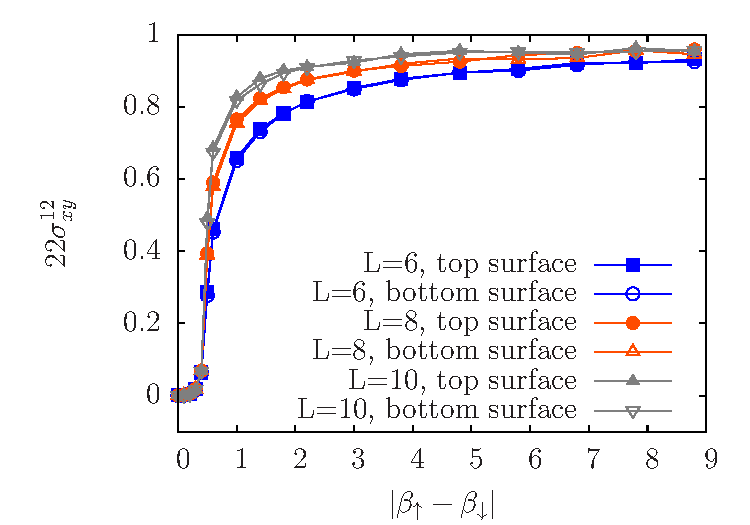
\includegraphics[width=0.9\linewidth]{figures/cp1hall.eps}
\caption{Hall conductivity on the surface of the $CP^1$ version of the model, in units of $e^2/h$. On each surface we find that the conductivity is quantized to $1$, and this odd-integer value shows that we are on the surface of a bosonic TI. Data was taken for $K=0.4$, $\lambda=8$, $\beta_\downarrow=\beta_{\rm bulk}=0.2$. We measure the same conductivity on both the top and bottom surfaces of the topological phase.}
\label{cp1hall}
\end{figure}

%%%%%%%%%%%%%%%%%%%%%%%%%%%%%%%%%%%%%%%%%%%%%%%%%%%
\section{Realizing a symmetry-enriched topological phase by binding multiple hedgehogs to a boson}
\label{section::multiple}

In all of the above sections, we have studied a system where a single boson is bound to a single hedgehog. In this section we will describe the additional physics which arises when our system contains bound states of multiple hedgehogs. We induce this multiple binding by making the following change to Eq.~(\ref{action}):
\begin{equation}
S=S_{\rm spin}+\frac{\lambda}{2}\sum_{r,\mu} [ dJ_\mu(r)- Q_\mu(r)]^2.
\label{cdbind}
\end{equation}
Here $d$ is an integer, and the action will bind a boson to $d$ hedgehogs. 

When $d\neq1$ the change of variables in Eq.~(\ref{shift}) can no longer be applied. Therefore the phase diagram in this case will be different from the $d=1$ case. We can determine the phase diagram by performing Monte Carlo simulations. As an example, the phase diagram for $d=3$ is shown in Fig.~\ref{fracphase}. Phase boundaries were determined from singularities in the specific heat. Note that in the Heisenberg model we can define a maximum of one hedgehog per lattice site, and so this model cannot easily be used to describe the binding of  multiple hedgehogs. Therefore all results for $d \neq 1$ come from the $CP^1$ model. 

The phase diagram in Fig.~\ref{fracphase} is presented in terms of the variables $\lambda$ and $K$, with $\beta=0.1$. 
At small $\lambda$ and $K$, there is no energy cost for either hedgehogs or bosons, and they are independent. This leads to a paramagnet of spins and a superfluid of bosons. The spin $U(1)$ symmetry is preserved, and the boson $U(1)$ symmetry is broken. In contrast, at large $\lambda$ and $K$ both hedgehog and boson currents are forbidden, leading to a Coulomb phase of spins and an insulator of bosons. Here both the spin $U(1)$ symmetry and the boson $U(1)$ symmetry are preserved, but the spins have intrinsic topological order. At large $K$ but small $\lambda$, both symmetries are broken, while at very small $K$ and large $\lambda$ neither symmetry is broken, and we are in the binding phase. The phase diagram for $d=1$ contains only these four phases. For $d=1$ these are the only phases, and due to the change of variables in Eq.~(\ref{shift}), the phase transitions are all straight lines.
\begin{figure}
\includegraphics[angle=-90,width=0.9\linewidth]{figures/fracphase.eps}
\caption{Bulk phase diagram for the model described in Eqs.~(\ref{sspin}) and (\ref{cdbind}), with $d=3$. We can compare this to the case of $d=1$, where the middle phase is absent, and to $d=2$, where the middle phase is absent and there is a line of phase transitions between the paramagnet/superfluid and the Coulomb phase/insulator.}
\label{fracphase}
\end{figure}

 With $d\neq 1$, we have a new phase in the middle of the diagram, and no direct transition from the phase in the lower right to the binding phase. The middle phase can be understood as one in which hedgehog currents have proliferated, but the potential that they see is still too high for objects with three hedgehogs to exist. Therefore bound states are not possible and the boson currents stay gapped. Like the binding phase, this phase preserves the $U(1)$ symmetries from both the bosons and the spins. The topological phase only arises when $K$ is lowered to the point that objects with a hedgehog current of $3$ are proliferated, at this point bound states can form and the system becomes topological. For other values of $d$, the phase diagram is expected to have a similar form, with the exception of $d=2$, where the middle phase is absent and there is a line of phase transitions between the lower left and upper right phases. 
%For $c\neq 1$, $d\neq 1$, the phase diagram can have a more complicated form. 

For $d>1$, the phase at large $\lambda$ and small $K$ is a `binding' phase which binds $d$ hedgehogs to a boson. This phase is distinct from the topological phase discussed earlier in this work. In particular, it has intrinsic topological order. Condensing bound states of $d$ hedgehogs causes the electric field lines in the phase to fractionalize, i.e. it is possible to have electric field lines of strength $1/d$. These fractionalized electric field lines are one of the gapped excitations of the system. The other elementary gapped excitation the other is a single hedgehog, which binds to a boson charge of $1/d$. The hedgehog has well-defined statistics as it encircles the electric field lines, and we expect it to acquire a phase of $2\pi/d$ when this happens. The matter fields ($\phi_\uparrow$ and $\phi_\downarrow$) act as sources and sinks for electric field lines of integer strength, therefore the topological excitations in the system are only defined up to an integer, and we can say that the system has $\mathbb{Z}_d$ topological order.


The Witten effect and Hall effect measurements can be extended to the cases with multiple hedgehogs. For the Witten effect, the amount of bound charge will be modified, since now each hedgehog carries a charge of $1/d$. Therefore the screening cloud will have a charge of $1/(2d)$. We have studied the cases of $d=2,3$ in Monte Carlo and our results confirm this expectation. 
%This is not surprising, since in this case we do not have a topological phase. The reason there is no Witten effect is that the half hedgehog bound to the external monopole carries an integer amount of boson charge. This charge can be screened by other charges in the system. Note that with different choices of non-universal parameters, it would also be possible to observe an integer amount of bound charge. It is the binding of precisely one half of a charge that is the indication of topological behavior.
Our results for the Hall conductivity are shown in Fig.~\ref{halldiff}. We find that the surface Hall conductivity is given by $1/d$, which is one-half of the value found for a two-dimensional bosonic fractional quantum Hall effect.
%This does not indicate that the system is topological, since we could place a $2$ dimensional bosonic SPT on the surface of a trivial insulator and get the same result. Only a fractional Hall conductivity is an indicator of topological behavior. 

\begin{figure}
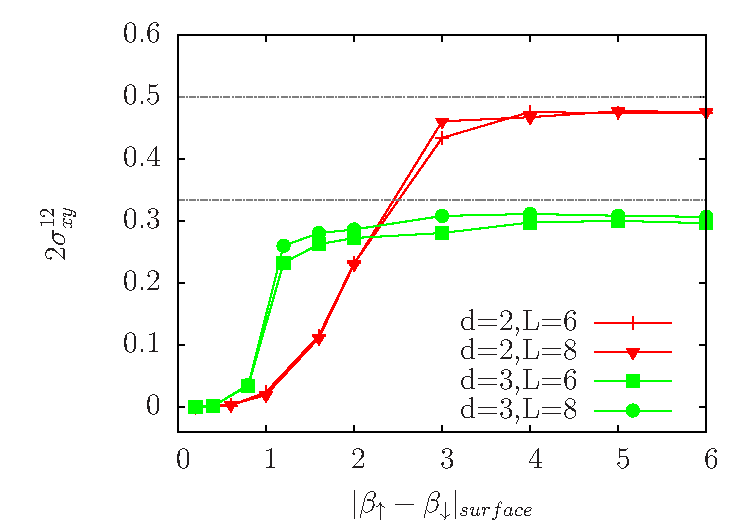
\includegraphics[width=0.9\linewidth]{figures/halldiff.eps}
\caption{Surface Hall conductivity for diffent values of $d$, in units of $e^2/h$. We see that the Hall conductivity is given by $1/d$. Both surfaces have been averaged over to improve statistics. Dashed lines are drawn at $1/d$ to guide the eye. Data was taken with $K=0.2$, $\lambda=8$. Different values of $\beta$ were used for different values of $d$, since the phase diagram changes as $d$ changes (see for example Fig.~\ref{fracphase}) and $\beta$ needs to be chosen so that the system is in the topological phase.}
\label{halldiff}
\end{figure}


\section{Discussion and Conclusions}
%discussion of charges bound to monopoles (connections with Matthew)

\bibliography{SO34D}
\end{document}
